% Аутоматски генерисано из Увод у пословну интелигенцију.docx

\chapter{Увод у Пословну интелигенцију}
\label{ch:uvod}
Од када људи одлучују била им је потребна одређена подршка у том процесу. Подршка одлучивању је потребна из најмање три разлога:

1. У скоро свим ситуацијама одлучивања постоји велика количина података коју је потребно обрадити, а да би се обрадио постојећи обим података потребна је и сразмерна количина времена.

2. Време за одлучивање је увек ограничено, тј. постоји временски период у коме је потребно донети одлуку. Овај период је, по правилу, увек мањи од периода који је потребан да би појединац обрадио све податке који му стоје на располагању.

3. Постоји потреба доносилаца одлуке (ДО) да донесу исправну одлуку како би организација остала конкурентна и успешно остваривала своје циљеве.

Због претходно наведених ограничења данас подршка одлучивању не може да се замисли без употребе информационих технологија и система.

За подршку одлучивању у организацијама у данашње време се најчешће користи назив Пословна интелигенција (енгл: \textit{Business Intelligence}, може да се преведе и као пословно обавештавање). Пословна интелигенција може да се дефинише као:

\textbf{Скуп информационих система, знања и вештина ДО у организацији удружених у генерисању, интеграцији и моделирању одлучивања са циљем да се дође до знања потребног за доношење одлука.}

Под пословном интелигенцијом се најчешће подразумевају две технологије:

1. Складиштење података (енг. Datawarehousing) које ће бити обрађено у другом поглављу књиге и

2. Откривање законитости у подацима (енг. Data Mining) које ће бити обрађено у трећем поглављу.

У овом делу поглавља се описују информациони системи који су претходили системима пословне интелигенцији, а то су системи за подршку одлучивању (СПО), групни системи за подршку одлучивању (ГСПО) и експертни системи (ЕС).

Да би се разумела подршка одлучивању најпре је неопходно позабавити се тиме где се она примењује, тј. за које одлуке је она ефикасна. Тако ће бити показано да за оперативне одлуке није неопходна подршка одлучивању, док је за тактичке и стратешке одлуке подршка одлучивању пожељна.

Одлуке које се доносе у организационом окружењу могу бити:

\begin{itemize}
  \item Оперативне: Најчешће извршаване одлуке које карактерише могућност довођења до потпуне аутоматизације, због учесталости извршавања и због своје „структурираности“. Код оперативних одлука је најбитнија метрика ефикасност њиховог извршавања.
  \item Тактичке: Одлуке извршаване на средњем нивоу менаџмента. Представљају спону између оперативних и стратешких одлука. Њихова улога је да омогуће превођење стратешких у оперативне одлуке. Пошто је пресудно доносити исправне одлуке на овом нивоу, нагласак је на ефективности ових одлука.
  \item Стратешке: Представљају најсложеније одлуке које треба донети. За њихово доношење и реализацију је потребно највише времена. У хијерархији одлука заузимају челно место и најзанимљивије су за анализу. Ове одлуке доносе најискуснији менаџери.
\end{itemize}
Претходно наведена хијерархија одлука описана је на слици 1.1. (Сукновић и други, 2021)

\begin{figure}[h]
    \centering
    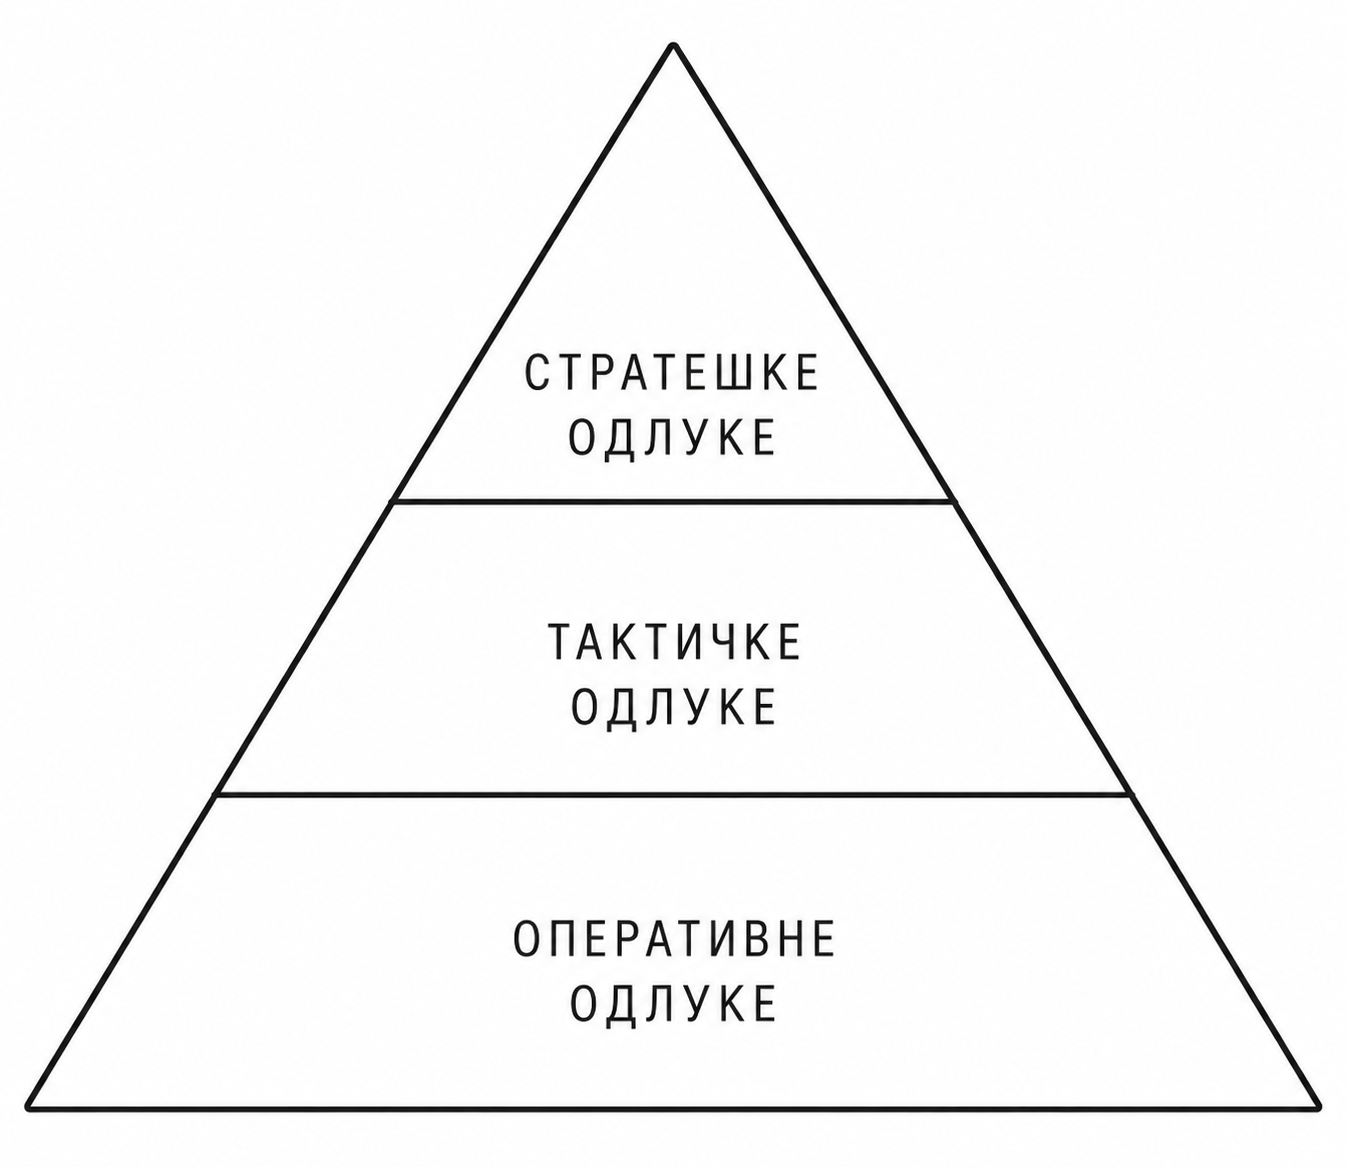
\includegraphics[width=0.85\linewidth]{slike/01/01-09.png}
    \caption{Хијерархија одлука}
    \label{fig:01-1}
\end{figure}

Подршка одлучивању се првенствено користи на стратешком и тактичком нивоу доношења одлука. Пошто су оперативне одлуке устаљене, оне могу да се аутоматизују, те подршка одлучивању код њих није неопходна.

Следи неколико примера у којима се користи подршка одлучивању.

\textbf{Пример 1 (Одлив клијената).}

Компаније све више занима да управљају животним циклусом својих потрошача и да препознају ситуације у којима долази до незадовољства клијента и потенцијалног одласка. Ово се односи на банке, телекомуникационе компаније, али све више и на универзитете који су заинтересовани да уоче ако постоје тешкоће у учењу студената и потенцијалном доношењу одлуке о прекиду студија. Ако се на време препозна намера одласка клијента, може на време и да се предупреди таква одлука.

\textbf{Пример 2 (Хипермаркети).}

Велике продавнице робе широке потрошње желе да сазнају како да што ефикасније управљају својом продајом. Да би то урадили они анализирају узоре продаје артикала како би што боље спознали потрошачке навике и на основу тога доносили одлуке које им могу донети још већу добит.

Проблеме из наведених примера је врло тешко решити без подршке одлучивању и система пословне интелигенције, због захтева за сагледавањем велике количине података, правовременим и исправним одлукама.

Треба напоменути да као што је одлучивање иманентно свим функцијама савременог менаџмента, тако је и подршка одлучивању постала саставни део сваког управљања организацијама заснованог на информационим системима.

\textbf{Подршка одлучивању је интердисциплинарна научна област коју подупире доношење одлуке у различитим менаџмент и бизнис функцијама, као што су маркетинг, финансије, управљање људским ресурсима, управљање производњом, итд.}

\section{Структурираност проблема}
Циљ развоја сваког модела за подршку одлучивању је развити структуриран модел. Тактичке и стратешке одлуке су обично полуструктуриране и неструктуриране. По Сајмону (Херберт А. Сајмон, добитник нобелове награде из економије 1978. године у области истраживања доношења одлуке у организацији), структурираност проблема се може изједначити са његовом дефинисаношћу, а под потпуно дефинисаним (структурираним) проблемом подразумева се да:

1. је проблем јасан,

2. су прецизно дефинисани улазни подаци и

3. су познати начини на који се врши анализа и долази до решења.

Проблеми које је потребно решавати са становишта одлучивања могу бити структурирани, полуструктурирани и неструктурирани. Када је проблем структуриран њега је могуће релативно лако дефинисати, док је за преостала два случаја то значајно теже. У случају неструктурираности ради се о одсуству свих горе наведених елемената, док за полуструктурираност неки од елемената структурираности недостају. Мало аутора се упушта у прецизно дефинисање тих случајева, а ретки су се одлучили да их објасне на свакодневним примерима, као што су то учинили (Leigh \& Doherty, 1986). Због тога се неки њихови примери и наводе у Табели~\ref{tab:01-1}

\begin{table}[h]
\centering
\begin{adjustbox}{max width=\textwidth}
\begin{tabular}{|l|l|l|}
\hline
\textbf{СТРУКТУРИРАНИ ПРОБЛЕМИ} & \textbf{ПОЛУСТРУКТУРИРАНИ ПРОБЛЕМИ} & \textbf{НЕСТРУКТУРИРАНИ ПРОБЛЕМИ} \\
\hline
Открити минус у чековној књижици & Наћи неубележени депозит у књижици & Обезбедити се од таквих проблема у будућности \\
\hline
Возити кола кући & Установити да постоји мали квар на колима & Одржавати кола тако да се не кваре \\
\hline
Израчунати рату за кола & Наћи банку која ће позајмити новац & Постати довољно богат да зајам није потребан \\
\hline
Израчунати цену трансакције са акцијама на берзи & Изабрати групу акција које задовољавају неке критеријуме инвестирања & Тачно предвидети акцију берзе за наредни дан \\
\hline
Попунити кратки формулар & Одредити политику цене за плаћање пореза & Преправити формуларе за плаћање пореза \\
\hline
\end{tabular}
\end{adjustbox}
    \caption{Примери нивоа структурираности проблема}
    \label{tab:01-1}
\end{table}

Занимљиво је да 40 година након објављивања ове табеле, за све од наведених изазова у Табели~\ref{tab:01-1} постоје системи који пружају подршку одлучивању. То су редом: Системи електронског банкарства, Системи превентивног одржавања возила, Електронски инвестициони саветници, Берзански предиктивни системи, Системи за помоћ при попуњавању и преправљање пореских формулара. Оно што је пре 40 година деловало као научна фантастика данас је постала реалност.

Табела~\ref{tab:01-1} представља гледиште поменутих аутора на проблем структурираности. Структурираност се мери у односу на степен знања који ДО поседује о одређеној области. Наиме, ако ДО влада знањем у одређеној области за њега су проблеми из те области структурирани. За ДО ван те области, проблеми су неструктурирани.

Да би ДО могао да решава пословни проблем, он за њега треба да постане структуриран, те је један од основних циљева подршке одлучивања:

\textbf{Превођење проблема одлучивања из неструктурираности у структурираност је неопходан услов за подршку одлучивању, а ово значи да се развије модел за подршку одлучивању.}

Ова једноставна замисао је код решавања реалних проблема прилично сложена. Ипак, од квалитета ове трансформације зависи и процес доношења одлуке.

Надамо се да ће кроз наставак ове књиге постати јасно на које начине може да се изврши ова трансформација и које су предности и недостаци метода које врше овај задатак.

Ако су примери из табеле 1.1. појаснили појам и проблем структурираности остаје да се види зашто је тај проблем интересантан и значајан у подршци одлучивању. Као што је већ напоменуто, у општој теорији одлучивања постоје три врсте одлука: стратешке, тактичке и оперативне. За оперативне одлуке се сматра да су потпуно структуриране, тактичке се крећу од потпуне ка делимичној структурираности, док су стратешке одлуке углавном неструктуриране или у најбољем случају полуструктуриране.

С друге стране, интересантан је однос информационих система, који се користе при одлучивању, према структурираности проблема. Класична обрада података и информациони системи су идеални за проблеме који су потпуно дефинисани (структурирани), док та констатација не важи за преостале случајеве. Како средње и највише руководство (менаџери) доносе тактичке и стратешке одлуке, произилази да су, поготово ови последњи, практично „остали“ без могућности ефикасне рачунарске подршке. Та чињеница је практично и довела до појаве система за подршку одлучивању, као првог „алата“ који се ухватио у коштац са неструктурираним проблемима. (Сукновић и Делибашић, 2010)

\section{Системи за подршку одлучивању}
Први системи који су се формално почели бавити подршком одлучивању као засебном научном дисциплином су системи за подршку одлучивању. Почеци система за подршку одлучивању (СПО) су везани за проучавање одлучивања у организацијама крајем 50-их и почетком 60-их година прошлог века. У седамдесетим годинама 20-ог века је почело и проучавање експертних система (ЕС). СПО и ЕС имају за циљ унапређење пословног одлучивања, а тај циљ остварују различитим приступима.

Најистакнутији аутор из дисциплине СПО (Turban et al., 2006) дефинише СПО преко већег броја дефиниција:

СПО је систем који треба да подржи управљачке одлуке у полуструктурираним и неструктурираним ситуацијама одлучивања.

СПО треба да буде помоћ ДО у смислу повећавања њихових способности, а никако као њихова замена.

СПО је рачунарски систем који пружа подршку при решавању полуструктурираних и неструктурираних проблема у процесу доношења одлука.

СПО пружа адаптиван и еволутивни процес који може помоћи ДО да боље разуме и анализира сопствени процес доношења одлука.

СПО је интерактивни рачунарски систем који користи језике програмирања четврте генерације и базе података за подршку решавању неструктурираних или полуструктурираних проблема у процесу доношења одлука руководства.

СПО су алати, или рачунарски системи који омогућавају бољу продуктивност ДО у процесу одлучивања.

Вишегодишњим изучавањем дисциплине СПО, (Сукновић и Делибашић, 2010) дају следећу дефиницију:

\textbf{СПО су информациони системи, који су слични и комплементарни стандардним информационим системима и имају за циљ да подржавају пословне процесе доношења одлука. Представљају симбиозу информационих система, организационог знања и процеса доношења одлука.}

Већ спомињани (Turban et al., 2006) такође наводи неке од особина СПО које су по њему значајне и које карактеришу сваки СПО:

1. СПО обезбеђује подршку доносиоцима одлука у полуструктурираним и неструктурираним ситуацијама кроз спајање људских процена и рачунарских информација.

2. Подршка је обезбеђена за различите нивое управљања, од највишег ка најнижем.

3. Подршка је обезбеђена како појединцима тако и групама. Шта више, СПО помаже интеграцију појединаца кад год је то потребно.

4. СПО обезбеђује подршку већем броју независних и/или секвенцијалних одлука.

5. СПО подржава све фазе процеса одлучивања: обавештавање, пројектовање, избор и примену (Simon, 1945).

6. СПО подржавају различите процесе одлучивања и различите стилове одлучивања.

7. СПО морају бити адаптивни у времену, а ДО мора бити у стању да реагује на све промене. То омогућава временски адекватне и брзе ad-hoc анализе.

8. СПО треба да буду једноставни за коришћење.

9. СПО треба да побољшају ефективност одлучивања (постизање циљева у посматраном временском периоду), пре него његову ефикасност (оптимизација трошкова одлучивања).

10. ДО има потпуну контролу над свим корацима у процесу одлучивања при решавању проблема. СПО треба да помогну, а не да замене ДО, који увек може да не прихвати сугестију добијену од СПО.

11. СПО треба да води ка учењу, што природно води ка новим унапређењима система, а што опет води ка новом учењу итд.

12. СПО морају бити једноставни за развој, тј. њих треба да могу да конструишу чак и ДО.

Сваки систем за подршку одлучивању се састоји из најмање три подсистема (Sprague \& Carlson, 1982), (Сл. 1.2):

1. Базе података,

2. Базе модела и

3. Корисничког интерфејса.

Подсистем базе података представља део СПО у коме се чувају улазни и излазни подаци организације. Међутим, код база података примењених у СПО постоје и извесне специфичности. Наиме, база података код СПО може да се разликује од релационих база података, о чему ће бити више речи у осталим поглављима ове књиге.

Подсистем базе модела представља компоненту СПО која се састоји од модела одлучивања. Сваки модел решава одређени проблем код одређеног пословног процеса. Њихов задатак је да на основу улазних података и модела одлучивања генеришу излазне податке на основу којих ДО може да доноси одлуке. Улазни, као и излазни подаци могу да се чувају у бази података.

Управљање моделима, као и избор одговарајућег модела, је код класичних СПО препуштен ДО. Типични модели који се налазе у бази модела СПО служе подршци решавању полуструктурираних и неструктурираних проблема одлучивања.

По поменутим ауторима кључне особине СПО у подсистему модела укључују способности:

1. укључивања нових модела у систем,

2. приступања и интеграцији „блоковима модела“ ради добијања новог модела,

3. каталогизирања и одржавања широког опсега модела за различите кориснике,

4. повезивања ових модела са одговарајућим везама у бази података и

5. управљања базом модела.

Подсистем корисничког интерфејса по својој основној функцији треба да омогући (и то на што једноставнији начин) комуникацију између СПО и корисника. То је управо због ДО, који по правилу нису специјалисти за одређени модел, основни разлог због чега је овај подсистем и најважнији. СПО могу да користе како крајњи ДО, тако и аналитичари који припремају одлуке користећи СПО за ДО.

\begin{figure}[h]
    \centering
    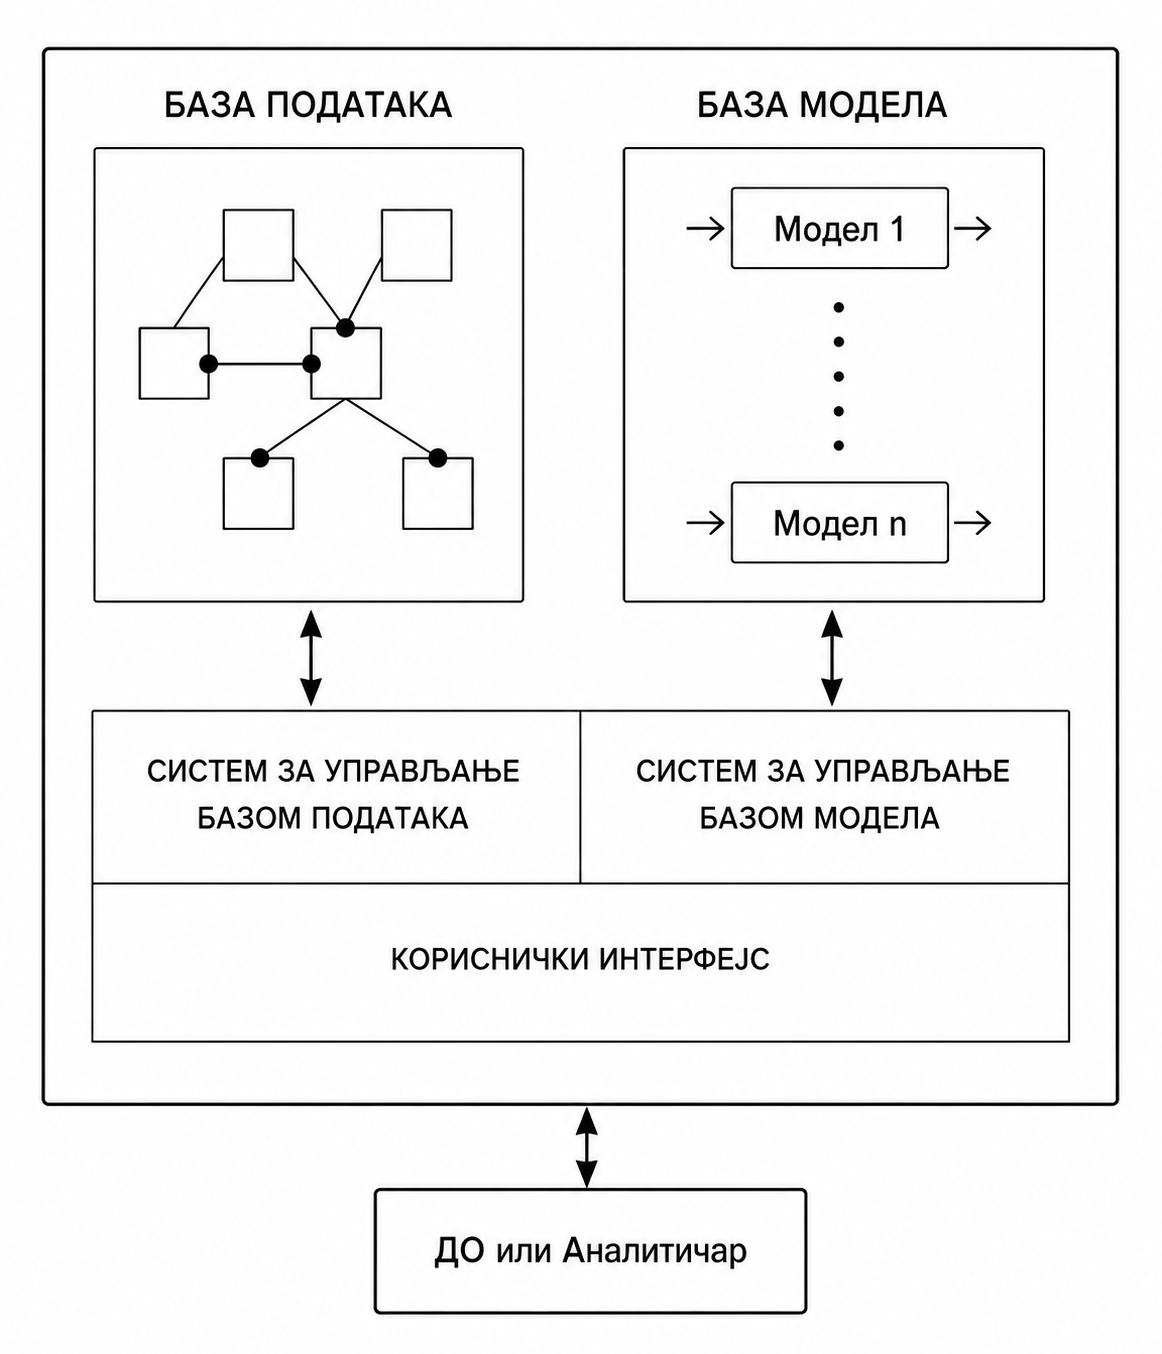
\includegraphics[width=0.85\linewidth]{slike/01/01-30.png}
    \caption{Компоненте СПО}
    \label{fig:01-2}
\end{figure}

У већини случајева се подсистем корисничког интерфејса састоји из три дела (Bennett, 1983):

1. језик акције: којим корисник комуницира са системом,

2. језик презентације: шта корисник види на интерфејсу и

3. база знања: шта корисник мора знати (о систему за подршку одлучивању).

(Turban et al., 2006) наводи сличну структуру архитектуре СПО и сматра да се сваки СПО састоји из следеће три компоненте:

1. Управљање подацима - укључује базе података са релевантним подацима за посматрану ситуацију и управљане софтвером, који се зове систем за управљање базом података (СУБП);

2. Управљање моделима - софтверски пакет, који укључује финансијске, статистичке, управљачке и друге квантитативне моделе и који систему даје аналитичке могућности као и одговарајуће управљање софтвером;

3. Комуникацијски подсистем (кориснички интерфејс) - преко кога корисник комуницира са СПО и управља њиме.

СПО нуди одређене предности када се уведе у организацију. Основне предности СПО, које је још давне 1981. године навео (Keen, 1981) су:

1. Повећавање броја алтернатива за разматрање у процесу доношења одлука;

2. Боље разумевање проблема који треба да се реши;

3. Бржи одговор на непредвиђене ситуације; тј. краће време потребно за доношење полуструктурираних и неструктурираних одлука;

4. Способност спровођења ad-hoc анализа;

5. Боље сагледавање проблема и учење;

6. Побољшана комуникација међу члановима тима који учествују у доношењу одлуке;

7. Побољшана контрола одлучивања;

8. Уштеда у трошковима;

9. Боље одлуке;

10. Ефикаснији тимски рад;

11. Уштеда у времену и

12. Боље искоришћење расположивих података.

Са друге стране, класични СПО имају и одређене недостатке којих сваки инжењер који уводи овај систем у организацијама треба да буде свестан. Недостаци који се наводе у наставку су само делимично решени, те су неки од њих и данас актуелни.

Основни недостатак СПО огледа се у чињеници да постоји проблем избора и коришћења модела из базе модела. Наиме, када СПО има само један модел, овај проблем не постоји, али најчешће то није случај. СПО, по правилу, увек на располагање ДО нуде више различитих модела за решавање истог проблема. ДО тада може да има недоумицу:

1. Који модел изабрати?

2. Како користити изабрани модел? (иако ово зависи од способности и вештине ДО, постоје захтеви да се постојећи модел унутар СПО приближи ДО који решава реалне проблеме. Најчешће је потребно прилагодити постојеће моделе и то је процес који отежава примену СПО).

3. Како решити проблем за чије решавање не постоји модел у бази модела?

Сматра се да се проблем управљања базом модела може решити коришћењем експертног система (потпоглавље 1.5). У сваком случају је потребно експертско знање за решавање напред набројаних недоумица. У наставку књиге биће предложена могућа решења.

Иако је СПО технологија деведесетих година 20. века достигла свој зенит, може да се каже да је наставила да се развија под другим називима. Наследник СПО је свакако ПИ, али су се упоредо развијали и други системи, пре свега системи вештачке интелигенције (ВИ) и машинског учења (МУ) (Делибашић и други, 2009), који су постали доминантни у пружању подршке одлучивању.

За обраду података код СПО, за разлику од класичне обраде података, неопходне су могућности спровођења „шта-ако“ анализе, анализе осетљивости и анализе достизања циља. Ове анализе су изузетно значајне у процесу доношења одлука.

Да би се појаснило место СПО у рачунарским и информационим наукама даје се преглед технологија које се користе за подршку одлучивању:

\begin{itemize}
  \item Управљање ресурсима предузећа – ЕРП (енг. Enterprise Resource Planning): информациони системи који подржавају трансакциону обраду података, прикупљају и складиште трансакционе податке организација и омогућавају процесну интеграцију података.
  \item Пословна интелигенција – ПИ: информациони системи који подржавају аналитичку обраду података, подаци из ЕРП система су пречишћени, интегрисани, и спремни за анализу. Корисницима су на располагању контролне табле, аналитичке коцке, пивот табеле, којима могу да навигирају кроз податке организације и праве, између осталог, и ad-hoc упите.
  \item Системи за подршку одлучивању – СПО: информациони системи који уводе додатне аналитичке капацитете са циљем да се подржи процес одлучивања. Уводи се димензија акција за одлучивања, које нису експлицитно биле изражене код ЕРП и ПИ. Подржавају се предиктивна аналитика, анализе осетљивости, противчињеничне анализе, моделовање сценарија, оптимизационе процедуре. Да би се испунили сви ови аналитички и одлучивачки захтеви користе се, између осталих, и методе ВИ и МУ.
\end{itemize}
Да би се предвидело како ће будућност система пословне интелигенције изгледати, треба се сетити генеричког оквира за развој СПО предложеног од стране (Holsapple \& Whinston, 1996), а приказаног на слици 1.4. Овај оквир пружа прилично стабилан поглед на технологију СПО, шта она представља и шта ће представљати и у времену које долази.

\begin{figure}[h]
    \centering
    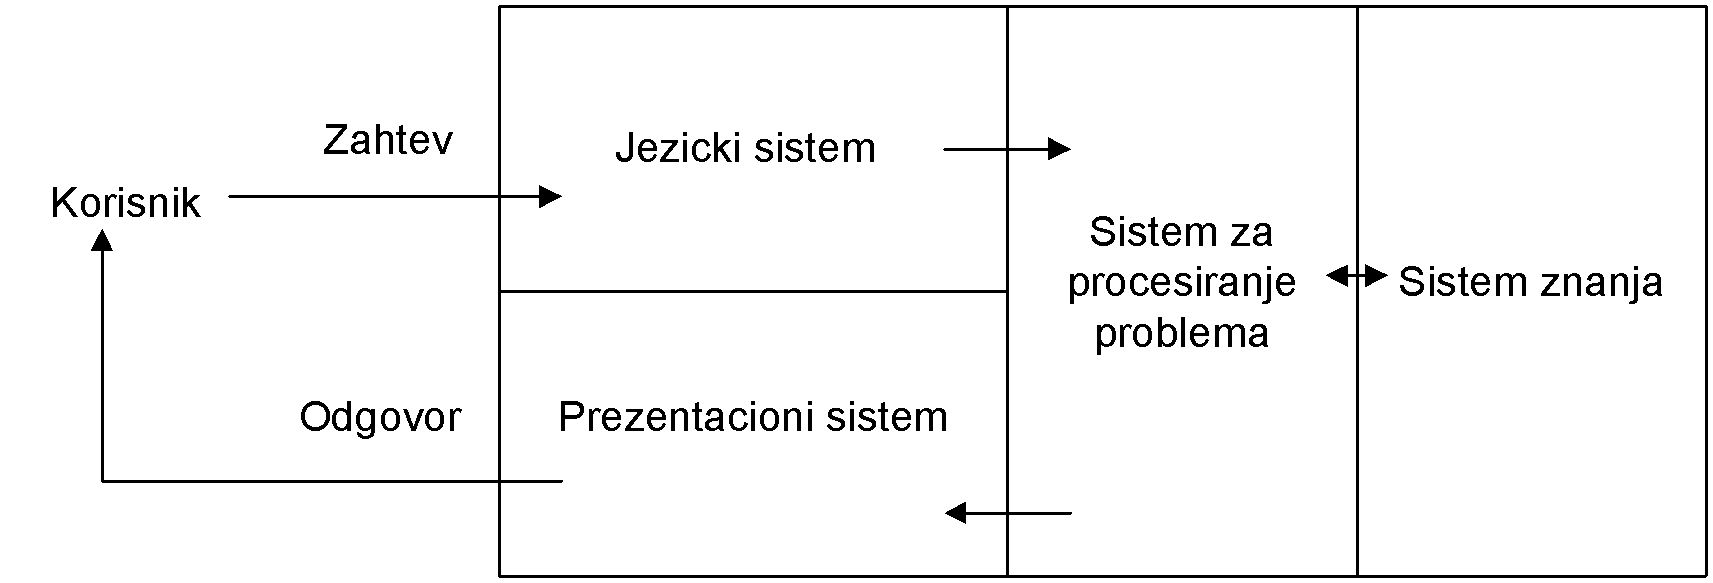
\includegraphics[width=0.85\linewidth]{slike/01/01-26.png}
    \caption{Генерички оквир СПО}
    \label{fig:01-3}
\end{figure}

Генерички оквир за развој СПО треба да омогући ефикасну комуникацију између ДО и података организације. Да би ДО из података добио одговарајућу подршку одлучивању најпре треба да има могућност да преко одговарајућег интерфејса (језички систем) пренесе свој захтев (дефинисан проблем) систему.

Након примљеног захтева систем треба да анализира проблем (систем за процесирање проблема). СПО на основу знања садржаног у систему и захтева корисника треба да генерише одговарајући одговор (предлог решења). Одговор кориснику на постављени захтев СПО омогућава преко презентационог система.

Већина СПО се и развија да садржи све компоненте система, међутим овакво гледање на СПО нам омогућава да посматрамо СПО као технологију која се може придодати свим организационим системима и тиме повећати квалитет доношења одлука.

\textbf{Као што је одлучивање иманентно свим функцијама организације, тако је и подршка одлучивању иманентна свим системима развијеним да подрже одлучивање у свим функцијама организације.}

Један поглед како би СПО могли да изгледају предложили су и (Azvine et al., 2006). Аутори описују како би СПО могао изгледати у будућности. СПО би, по наведеним ауторима, требало да задовољи следеће услове:

\begin{itemize}
  \item пуњење података у базу података у реалном времену,
  \item пуњење модела из базе модела у реалном времену,
  \item анализа резултата модела у реалном времену и
  \item доношење одлуке у реалном времену.
\end{itemize}
Да се СПО мењају потврђује и (Lawton, 2006), који наводи да је кориснички интерфејс система ПИ знатно побољшан у односу на претходни период, а неке апликације ПИ већ омогућавају рад у реалном времену.

Визија савремених система СПО је да се омогући функционисање система који ће омогућити пут од захтева за решењем до решења (информације са предлогом одлуке) без застоја и препрека, тј. у реалном времену. Да би се то постигло, процес доласка до знања (информација са предложеном акцијом одлуке) треба да се аутоматизује.

\textit{Данас, захваљујући напретку у облаку рачунарства (енг. Cloud Computing), платформама за обраду великих података (нпр. Apache Hadoop, Apache Spark) и самоуслужним БИ алатима (нпр. Power BI, Tableau, Looker), овај циљ је у значајној мери остварен. Савремени системи ПИ омогућавају корисницима да сами креирају извештаје и визуализације без потребе за специјализованим аналитичарима, чиме се драстично скраћује време од податка до одлуке. Додатно, примена машинског учења и вештачке интелигенције (укључујући и велике језичке моделе) аутоматизује многе кораке у аналитичком процесу.}

У наставку се приказују слојеви који чине структуру једног интегрисаног система пословне интелигенције (Слика~\ref{fig:01-4}). То су:

1. трансакциони (оперативни),

2. интегративни и

3. аналитички слој.

\begin{figure}[h]
    \centering
    
\includegraphics[width=0.85\linewidth]{slike/01/01-28.png}
    \caption{Три слоја пословне интелигенције}
    \label{fig:01-4}
\end{figure}

Трансакциони или оперативни слој генерише податке пословања. Систем ПИ треба да буде везан за овај слој, и то двоструко. Све што се дешава у текућем пословању организације треба да се очитава у складишту података, и са друге стране: одлуке донете на основу извештаја из аналитичког слоја треба да се одразе у оперативном слоју и повратно кроз сам систем ПИ. Да би ово било могуће потребно је укључити следеће функционалности у систем ПИ:

1. Организациони (пословни) процеси треба да буду снимани константно и подаци из тог процеса учитавани у складиште података и

2. одлуке које доноси ДО треба да утичу на сам пословни процес.

Други важан слој система ПИ јесте интегративни слој. Овај слој представља спону између модела и података пословања. Он треба да обезбеди квалитетне податке за аналитички слој. Да би овај слој функционисао у реалном времену треба да се омогући:

1. Једноставан приступ подацима пословања кроз дефинисано складиште података (тема поглавља 2),

2. дефинисан ток учитавања података из пословања у складиште података и

3. систем за управљање квалитетом података и решавање проблема неквалитетних података код процеса учитавања података у складиште.

Аналитички слој је одговоран за прављење извештаја за ДО, у њега су укључени алати за извештавање као и различити модели из базе модела (међу њима највише се истичу алгоритми за откривање законитости у подацима – ОЗП) чији је задатак да на основу захтева корисника и података из базе података реше захтев ДО.

Пошто су модели на основу којих се праве извештаји и даље прилично сложени, овај слој у великој мери зависи од способности аналитичара коме је, са друге стране, потребна одређена количина времена док састави извештај или примени одговарајући модел. Аналитичар због сложености свог посла често је био уско грло интегрисаног система пословне интелигенције, тј. време које је њему/њој било потребно да састави одређени извештај имало је директни утицај на време које је потребно да се ДО пружи подршка одлучивању.

Да би систем ПИ могао да функционише у реалном времену, потребно је знања аналитичара, тј. његова експертска знања, формализовати и аутоматизовати. Знање аналитичара је било потребно аутоматизовати да би се омогућио аутоматски избор модела као и њихова примена. У данашње време, развојем великих језичких модела и агентских модела ово се све више постиже тако што се аутоматски бирају и подешавају модели за одређени скуп података.

Избор одговарајућег модела треба да зависи од природе корисничког захтева и од података који стоје на располагању за решавање тог захтева. Аналитичар у систему будућности добија нову улогу. Он треба да изврши почетно подешавање параметара система и да током функционисања система врши промену параметара и адаптацију система током времена.

\begin{figure}[h]
    \centering
    
\includegraphics[width=0.85\linewidth]{slike/01/01-20.png}
    \caption{Систем пословне интелигенције у реалном времену}
    \label{fig:01-5}
\end{figure}

\section{Експертни системи}
Као алати који треба да симулирају знање експерта, експертни системи (ЕС) могу да се дефинишу као програми који користе људско знање ради решавања проблема који захтевају људску интелигенцију. Једна од најпотпунијих дефиниција за ЕС потиче од врсног познаваоца ове области, Едварда Фајгенбаума (са Универзитета Стенфорд (Stanford)):

\textbf{Експертни системи су интелигентни рачунарски програми који употребљавају знање и процедуре закључивања да би решили проблеме који су довољно тешки, те захтевају значајну људску стручност и вештину. Знање са додатком механизма закључивања за решавање тог проблема могу се сматрати моделом који симулира најбољег стручњака у тој области.}

Да би се решили сложени полуструктурирани и неструктурирани проблеми потребно је експертско знање. Један од поменутих сложених проблема јесте проблем избора и примене одговарајућег модела, поменутог као један од изазова код традиционалних СПО. Како је подршка одлучивања скупа, а неопходна, развијани су експертни системи са циљем да симулирају знање врхунског експерта, које је са друге стране, било потребно за решавање пословних проблема.

\textit{Напомена: Класични експертни системи засновани на правилима (енг. Rule-based expert systems) су данас у значајној мери замењени или допуњени системима машинског учења који аутоматски уче обрасце из података, или великим језичким моделима који управо симулирају знање врхунског експерта. Разумевање принципа експертних система је важно јер је то темељ на коме су настали савремени системи вештачке интелигенције, а њихови елементи се и даље се користе при решавању реалних проблема.}

\subsection{Архитектура експертног система}
Сваки ЕС се састоји из три основна дела (Слика~\ref{fig:01-6}). То су:

\begin{itemize}
  \item база знања,
  \item механизам закључивања и
  \item кориснички интерфејс.
\end{itemize}

\begin{figure}[h]
    \centering
    
\includegraphics[width=0.85\linewidth]{slike/01/01-22.png}
    \caption{Основна архитектура експертног система}
    \label{fig:01-6}
\end{figure}

База знања садржи знање експерта у рачунски читљивом формату.

Механизам закључивања има за циљ да на основу захтева корисника и знања у бази знања реши кориснички захтев, тј. да пронађе управо оно знање које је кориснику потребно. Механизам закључивања има две основне улоге:

1. испитује постојање одређеног знања у бази знања на основу корисничког захтева и проналази неопходно знање за решавање корисничког захтева и

2. уређују редослед кретања по бази знања у зависности од захтева корисника и структуре базе знања. Ово може бити и интерактиван процес.

Кориснички интерфејс треба да обезбеди једноставну комуникацију између система и корисника, тако што треба да омогући једноставну управљање експертним системом и квалитетну интерпретацију резултата.

\subsection{База знања}
База знања представља критични део експертног система. Због тога је поступак прикупљања знања од експерта, трансформација експертског знања у формални облик и организација базе знања најбитнији процес развоја експертног система.

База знања садржи законитости из специфичног домена знања које се моделирају. Постоје различити начини да се знање запише у читљивом облику за машине. Најпознатије методе представљања знања у бази знања су:

\begin{itemize}
  \item продукциона (ако-тада) правила,
  \item семантичке мреже,
  \item оквири знања,
  \item математичка (формална) логика,
  \item табеле одлучивања,
  \item дрво одлучивања, итд.
\end{itemize}
\textbf{Продукциона правила}

Представљају најчешће коришћени метод представљања знања. То су правила облика АКО услов ТАДА последица. Продукционим правилима се представљају логичке релације (везе) међу подацима. Овакав начин представљања знања је доста природан, а што је врло важно, има особину модуларности. Такође, задовољавају захтев за лаком модификацијом базе знања.

\begin{figure}[h]
    \centering
    
\includegraphics[width=0.85\linewidth]{slike/01/01-33.png}
    \caption{Однос правила и знања у радној меморији}
    \label{fig:01-7}
\end{figure}

\textbf{Семантичке мреже}

Знање представљају у облику мреже. Свака мрежа се састоји од чворова и веза међу чворовима. Везе исказују односе међу чворовима. Везе могу да приказују и наслеђивање међу чворовима.

\begin{figure}[h]
    \centering
    
\includegraphics[width=0.85\linewidth]{slike/01/01-31.png}
    \caption{Пример семантичке мреже}
    \label{fig:01-8}
\end{figure}

\textbf{Оквири знања}

Представљају скупове објеката, који се састоје од атрибута, где сваки атрибут има одређену вредност. Оквири знања представљају специјалан случај семантичких мрежа. Сваки оквир има статички део (подаци исти за класу објеката) и динамички део (подаци карактеристични за одређени објекат).

\begin{figure}[h]
    \centering
    
\includegraphics[width=0.85\linewidth]{slike/01/01-12.png}
    \caption{Пример оквира знања}
    \label{fig:01-9}
\end{figure}

\textbf{Математичка (формална) логика}

Код представљања знања математичком логиком, користе се најчешће две врсте логика: пропозициона логика и предикатски рачун. Пропозициона логика представља систем за закључивање у коме испитује да ли је одређена премиса тачна или није. Предикатски рачун представља проширење пропозиционе логике.

\textbf{Табела одлучивања}

Табела одлучивања представља још један вид чувања знања. Табела се састоји од атрибута и редова, а неки од атрибута могу садржати акцију одлучивања. Ове табеле представљају основни облик из којих алгоритми машинског учења развијају моделе, који даље могу да се употребљавају како у ЕС, тако и у другим СПО. Табела може да чува у себи или правила одлучивања или случајеве претходног искуства који су довели до одређене одлуке.

\begin{table}[h]
\centering
\begin{adjustbox}{max width=\textwidth}
\begin{tabular}{|l|l|l|l|l|l|}
\hline
\textbf{Дан} & \textbf{врем. прилике} & \textbf{температура} & \textbf{влажност} & \textbf{ветар} & \textbf{играти?} \\
\hline
1 & сунчано & Вруће & висока & слаб & не \\
\hline
2 & сунчано & Вруће & висока & јак & не \\
\hline
3 & облачно & Вруће & висока & слаб & да \\
\hline
4 & кишовито & Топло & висока & слаб & да \\
\hline
5 & кишовито & Хладно & нормална & слаб & да \\
\hline
\end{tabular}
\end{adjustbox}
    \caption{Скуп случајева одигравања утакмица за голф}
    \label{tab:01-2}
\end{table}

\textbf{Стабло одлучивања}

Стабло одлучивања чува знање у хијерархијском облику који је једноставно читљив. Оно може бити индуковано алгоритмима машинског учења из табела одлучивања, али исто тако може бити моделовано од стране експерта.

\begin{figure}[h]
    \centering
    
\includegraphics[width=0.85\linewidth]{slike/01/01-34.png}
    \caption{Стабло одлучивања за играње голфа}
    \label{fig:01-10}
\end{figure}

Овим свакако није исцрпљен преглед метода за чување знања. Треба имати на уму да се у решавању практичних проблема најчешће комбинује више различитих метода за представљање знања.

Без обзира на изабрани начин представљања знања, прикупљање истог је важна компонента приликом развијања експертног система. Овај посао поверен је такозваном инжењеру знања (\textit{knowledge engineer}), чији је задатак да успостави контакт са експертом и да запише знање експерта. Сам процес прикупљања знања од експерата назива се аквизиција знања (\textit{knowledge acquisition}).

\subsection{Механизам закључивања}
Представља део ЕС који има задатак да пронађе одговарајуће знање у бази знања и да га примени за решавање проблема. Захваљујући овом процесу каже се да су ЕС програми који се понашају „интелигентно“. Без механизма закључивања ЕС би био само енциклопедија, док је са механизмом закључивања ЕС деловао, у тадашње време, сличнији људском резоновању. Два су приступа у имплементацији механизама закључивања, и то: уланчавање унапред и уланчавање уназад.

\textbf{Уланчавање унапред}

Уланчавање унапред полази од премиса, АКО делова правила, у бази знања и упоређује их са чињеницама у меморији које је корисник изнео. Правила која су задовољена, могу се реализовати тако да се њихови ТАДА делови изврше. Ако се приликом претраживања покаже да ни једно правило није задовољено, ЕС закључује да нема довољно података да би проблем могао да се реши.

\textbf{Уланчавање уназад}

Уланчавање уназад је поступак обрнут од поступка уланчавања унапред. Код њега се полази од закључка, од ТАДА делова правила. Прво се претпостави да неко од могућих решења проблема важи и оно се означи као текућа хипотеза. Затим се проверава да ли важе све премисе тог правила. Овај поступак се рекурзивно понавља док год траје интеракција са корисником или док нема више правила у бази знања.

\subsection{Кориснички интерфејс}
Трећа, али подједнако значајна, компонента код ЕС је кориснички интерфејс. Основна улога овог елемента је да омогући рад корисника са експертним системом.

Поред дизајна, који је значајан за коришћење ове компоненте, изузетно је битно да корисник може:

1. јасно да изнесе свој кориснички захтев и

2. јасно да разуме резултате које му враћа систем.

Након представљања две различите технологије за подршку одлучивању, СПО и ЕС, следи потпоглавље о могућности комбиновања ова два приступа.

\section{Интеграција СПО и ЕС}
Успешна интеграција СПО и ЕС представља додатно побољшање оба приступа, у односу на ситуације када се они користе појединачно. Интеграцију ЕС и СПО је теоријски, а у неким случајевима и практично, могуће извести на пет различитих начина.

По (Turban \& Carlson, 1989) могуће комбинације „прикључења“ експертних система на системе за подршку одлучивању, се могу свести на неке типичне случајеве приказане на слици 1.13.

1. ЕС\#1 и ЕС\#2 уносе елементе интелигенције у системе за управљање базама података и модела, што је посебно значајно у овом другом случају.

2. ЕС\#3 има за циљ помоћ при коришћењу корисничког интерфејса.

3. ЕС\#4 и ЕС\#5 су замишљени као консултантска помоћ како градитељима СПО тако и њиховим корисницима.

\begin{figure}[h]
    \centering
    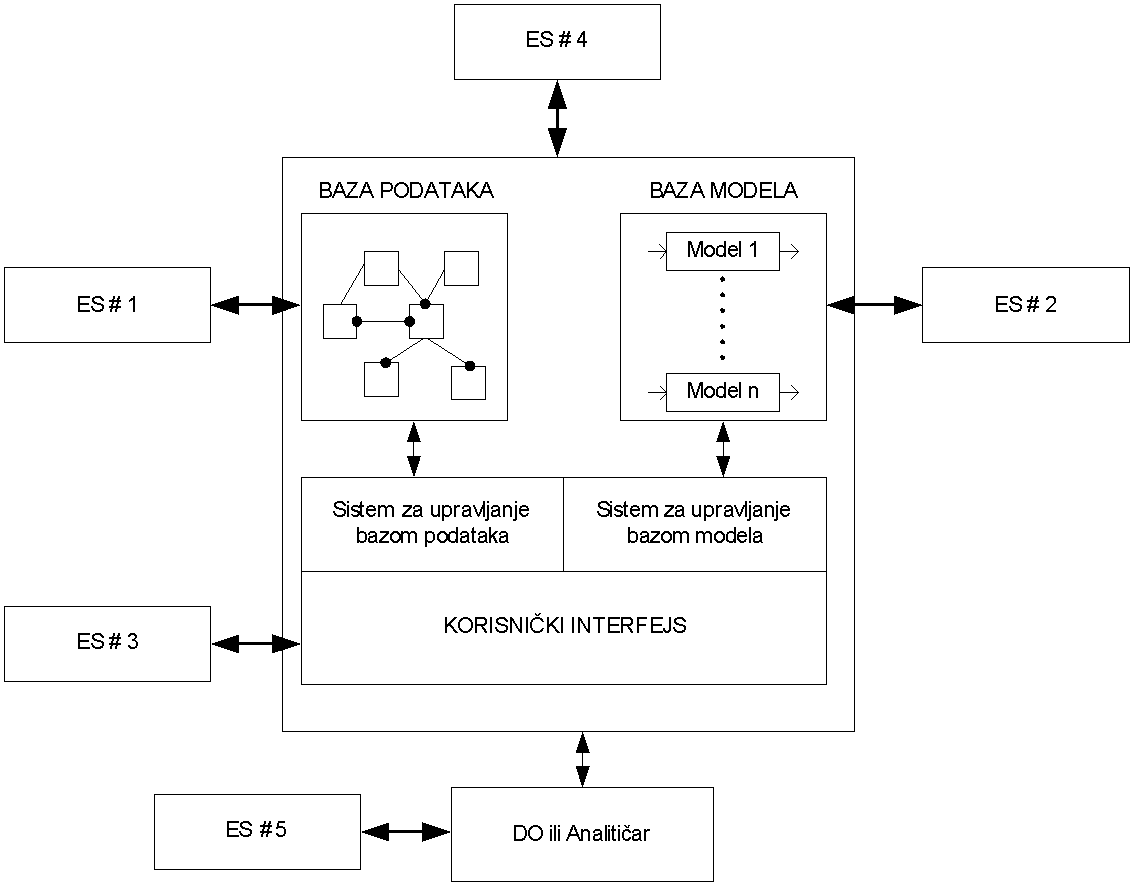
\includegraphics[width=0.85\linewidth]{slike/01/01-13.png}
    \caption{Могућности прикључења ЕС на СПО}
    \label{fig:01-11}
\end{figure}

Сви наведени начини прикључења решавају неки значајан проблем код развоја или коришћења СПО. Данас се све више, уместо ЕС, користе и друге технологије за решавање истих проблема. Пре свега се мисли на откривање законитости у подацима (ОЗП), велике језичке моделе и агентске системе.

По (Turban \& Carlson, 1989) ЕС је могуће придодати и као посебну компоненту СПО. Развијено је неколико могућности:

1. Излаз ЕС као улаз у СПО: Овај приступ је нарочито интересантан за почетне фазе процеса одлучивања.

2. Излаз СПО као улаз у ЕС: Овај приступ је посебно популаран јер експертним системима омогућује коришћење резултата различитих квантитативних анализа.

3. Повратна спрега: Представља комбинацију прва два приступа.

(Meader et al., 1984) су пошли од анализе процеса одлучивања и закључили да је већину уобичајених корака у том процесу могуће подржати типичним СПО функцијама. За кораке који подразумевају коришћење процена и креативности, они предлажу употребу ЕС.

(Roland, 1982) је уочио да ће СПО тешко моћи да доносиоцу одлуке сугеришу алтернативне акције које треба разматрати при одлучивању (фаза пројектовања по Сајмону), док ће бити у стању да кориснику помогну при евалуацији и избору између потенцијалних акција (фаза избора при одлучивању). Са степеном развоја данашњих технологија, ово више није немогуће, већ врло извесно.

До сада су разматрани системи за подршку одлучивању и експертни системи који превасходно подржавају индивидуално доношење одлука. Међутим, као што је већ напоменуто у особинама СПО (особина 3), подршка одлучивању није ограничена само на појединца – она треба да подржи и групно доношење одлука. У савременим организацијама, већину сложених одлука доносе групе људи, које су све чешће просторно и временски раздвојени. Из тог разлога, развијени су специјализовани системи који проширују концепт индивидуалног СПО на групни контекст. У наредним потпоглављима биће представљени алати за подршку рада групе и групни системи за подршку одлучивању (ГСПО), који омогућавају ефикасно колаборативно доношење одлука.

\section{Проблем базе модела код СПО}
Експертни системи поред основне намене, чување знања експерата, имају још неколико важних особина када се посматрају у односу на СПО (Сукновић и Делибашић, 2011):

1. Интеграцијом ЕС у СПО значајно се побољшава проблем управљања базом модела СПО.

2. Успешно реализована интеграција ЕС и СПО, представља први корак у креирању нових врста информационих система као што су: Информациони системи за извршне руководиоце (Executive Information Systems), Системи за подршку извршних руководиоца (Executive support systems), Системи за подршку менаџменту (Management support systems), итд.

Први који су у терминологију СПО увели појам базе модела су били (Sprague \& Carlson, 1982). Они су тада правилно уочили да процес креирања модела мора бити флексибилан, обављен са формалним језицима за моделирање и скупом „блокова за градњу“, који подсећају на потпрограме које је могуће склопити у циљу процеса моделирања.

У реализацији такве жеље није постигнут очекивани резултат. По мишљењу аутора ове књиге исувише истраживачког времена је изгубљено у покушају да се прекопира концепт управљања базама података на управљање базама модела. Данас је очигледно, да се радило о практично немогућем задатку, због фундаменталне разлике између података и модела.

Многи аутори су се бавили проблематиком управљања моделима. (Turban et al., 2006) је дао вероватно најпотпунији приказ оног што се под управљањем моделима подразумева (Слика~\ref{fig:01-12}).

\begin{figure}[h]
    \centering
    
\includegraphics[width=0.85\linewidth]{slike/01/01-23.png}
    \caption{Структура управљања моделима код СПО}
    \label{fig:01-12}
\end{figure}

Објашњавајући БМ и СУБМ, Турбан слично размишља као Спраг и Карлсон. Међутим, интересантна су размишљања о улози адресара модела, која по Турбану треба да буде специфичан каталог свих модела лоцираних у бази модела. Адресар треба да садржи дефиниције модела и његове основне функције, како би одговорио на корисникова питања везана за могућности коришћења и особине модела. Но, и поред тога адресар модела не даје одговор на суштинско питање: „Који модел треба користити, за коју прилику и потребу?“ На исто питање свој одговор не дају ни системи за управљање базом модела (СУБМ), јер да би се такав одговор уопште и могао дати, неопходно је поседовати експертска знања. По Турбану, таква једна чињеница представља и основни разлог за интеграцију експертних система у проблематику управљања моделима СПО.

Последња компонента структуре управљања има три функције:

\begin{itemize}
  \item Извршење модела - контролише извршавање модела.
  \item Интеграција модела - комбинује операције већег броја модела, када је то потребно. Посебно важну улогу у тој интеграцији има коришћење одговарајуће семантике.
  \item Процесор команди се користи за прихватање и интерпретирање моделских инструкција онако како теку од корисничког интерфејса ка СУБМ, извршавању модела и интеграцији модела.
\end{itemize}
Проблем управљања моделима у себи садржи још један суштински проблем. Ако би база модела била „велика“, тј. ако би у себи имала већи број модела, онда би практично корисник морао да их зна све, како би их могао најефикасније и употребити. Но, то је практично немогућ задатак, чак и за експерта из области.

Због тога је било потребно развити специјализовани експертни систем за избор модела из базе модела код СПО. Такав систем је требало да омогући кориснику да кроз неколико корака врши „тријажу“ модела, тј. одбацивање оних модела из базе модела који сигурно нису кандидати да буду коришћени.

Предност оваквог приступа је очигледна. Пре свега није неопходно суштинско познавање већег броја модела, што је по правилу случај када су у питању менаџери тактичког и стратешког нивоа, а они представљају најчешће крајње кориснике оваквих система.

Основни недостатак овог приступа је лежао у чињеници да је било немогуће пројектовати експертни систем којим би се решио проблем општег управљања моделима сваког СПО. За сваку конкретну ситуацију би се морао пројектовати одговарајући ЕС.

\section{Групно одлучивање}
У модерним условима пословања, већину сложених одлука у организацијама доноси специјализована група. Пораст сложености организационог одлучивања утицао је на раст потреба за честим састанцима и групним радом при чему су групе све чешће просторно и/или временски раздвојене (Сукновић и Делибашић, 2011).

Још почетком 2000-их година истраживања су показала да се значајан део сарадње међу запосленима одвија на различитим местима и у различито време. Од тада, овај тренд се драматично убрзао, посебно након глобалне пандемије COVID-19, када је рад на даљину (енг. remote work) и хибридни модел рада постао стандард у многим организацијама. Данас, у већини модерних организација, више од половине колаборације одвија се уз помоћ дигиталних алата, без физичког присуства свих учесника.

Подршка групном раду где чланови тима могу бити на различитим местима и да раде у различито време наглашава важне аспекте комуникације, компјутерских технологија и методологија рада. Ефикасни компјутерски алати за подршку рада групе (енг. groupware) су развијени да би смањили трошкове и омогућили ефикасну размену мишљења, информација, података, знања, докумената и других ресурса који су потребни за рад раздвојених група и/или појединаца. Ови алати могу подржати процес пословног одлучивања:

\begin{itemize}
  \item Индиректно – обезбеђују ефикасну колаборацију уз помоћ технологија као што су имејл (е-пошта), чет, дељење датотека, итд. Међутим ови алати не обезбеђују моделе одлучивања, као ни структуриран процес доношења одлука.
  \item Директно – обезбеђују структуриран и усмерен процес доношења одлука и интегрисане моделе и методе одлучивања чиме се омогућује генерисање решења за конкретан проблем (ГСПО).
\end{itemize}
У наставку ће бити описана оба типа алата за подршку одлучивању. Прво следи објашњење појма колаборације, компјутерских технологија које подржавају колаборацију, као и различити начини класификација ових технологија. Затим се детаљно описују групни системи за подршку одлучивању.

\section{Колаборативни алати за индиректну подршку одлучивању}
Колаборација или сарадња, представља комуникацију и координацију јединица унутар групе ради постизања заједничког циља. Јединице могу бити људи који чине тим, повезане организације, земље, заједнице, рачунари, роботи, итд.

У данашњим условима пословања неопходно је користити технологије (најчешће дигиталне) које омогућавају ефикаснију и ефективнију колаборацију, а самим тим и постизање циљева групе. Неке од технологија су: имејл, веб сајтови, тренутне поруке (енг. Instant messaging - IM), чет, е-групе, вики (енг. wiki) сајтови, форуми, дељени документи, дељене апликације, системи за управљање задацима и пројектима, виртуелне собе за састанке, итд.

У (Сукновић, 2001) предложен је временско-просторни оквир за класификацију алата за подршку рада групе (слика 1.15):

\textbf{Исто време/исто место (нпр. соба за одлучивање)}

Учесници се налазе у исто време на истом месту, као на традиционалним састанцима.

\textbf{Исто време/различито место (нпр. телеконференција)}

Учесници се налазе на различитим местима али комуницирају у исто време.

\textbf{Различито време/исто место (нпр. локална рачунарска мрежа)}

Учесници раде у сменама. Једна смена оставља информације наредној.

\textbf{Различито време/различито место (нпр. удаљено одлучивање)}

Учесници се налазе на различитим локацијама и деле информације асинхроно.

\begin{figure}[h]
    \centering
    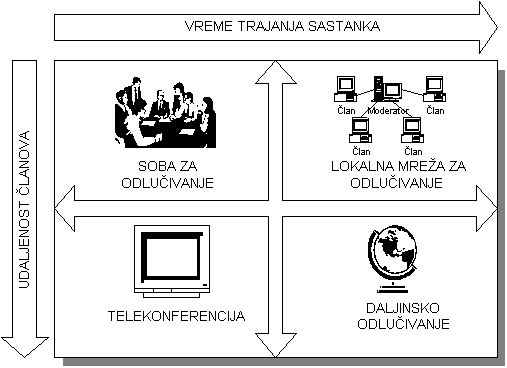
\includegraphics[width=0.85\linewidth]{slike/01/01-27.png}
    \caption{Врсте ГСПО апликација на основу критеријума удаљеност чланова-време трајања састанка}
    \label{fig:01-13}
\end{figure}

Технологије комуникације, зависно од природе проблема који помажу, могу се класификовати на:

\begin{itemize}
  \item синхроне и асинхроне,
  \item трајне (перзистентне) и привремене, и
  \item са кардиналношћу 1-1, 1-М, М-М.
\end{itemize}
Синхрони облици комуникације захтевају од свих учесника да истовремено буду присутни док се комуникација одвија. У ту класу би спадали: тренутне поруке, аудио/видео конференције, четови, итд.

Асинхрони облици омогућују учесницима да у различито време шаљу и примају поруке. У ове облике се могу сврстати: веб сајтови, е-пошта, форуми, итд.

Перзистентни облици комуникације чувају поруке на дуже време лако доступним. Од технологија за пренос трајних порука могу се користити веб и вики стране, дељени документи, итд.; док за привремене поруке могу да се користе форуми, е-групе, чет, имејл, итд.

Додатно, проблеме комуникације можемо поделити на оне који преносе поруке између два члана (1-1); између једног и више чланова (1-М); или поруке које више чланова преноси до више примаоца (М-М).

\section{Групни системи за подршку одлучивању}
Јака експанзија развоја информационих технологија, и уклањање временско-просторних баријера уз помоћ колаборативних алата, омогућили су развој групних система за подршку одлучивању (ГСПО). Прва истраживања у свету на ову тему заслуга су (Zelenny, 1982) са акцентом на употребу разноврсних модела групног одлучивања. Темеље за будућа истраживања поставили су (DeSanctis \& Gallupe, 1987).

\textbf{Групни системи за подршку одлучивању су интерактивни системи базирани на употреби информационе технологије и прецизног алгоритма одлучивања, а изграђени су на идеји индивидуалног (појединачног) СПО. Њихов основни задатак је да олакшају решавање полуструктурираних и неструктурираних проблема заједничким радом групе.}

Према (Theireuf, 1989), „ГСПО има за циљ да побољша групно одлучивање, уклањањем уобичајених комуникационих баријера, пружањем техника за структурирање анализе одлучивања и системско одређивање начина, времена и садржаја дискусије у циљу добијања већег квалитета одлуке“.

Битне карактеристике ГСПО, према (Сукновић, 2001) су:

\begin{itemize}
  \item ГСПО је посебно дизајниран систем, а не само склоп постојећих система.
  \item ГСПО је пројектован са циљем да помаже доносиоцима одлука у њиховом раду.
  \item ГСПО усклађује знања различитих корисника, те уз примену рачунара, омогућује бољу подршку одлучивању.
  \item ГСПО може бити специфичан (дизајниран за један тип проблема) или општи (дизајниран за различите одлуке на нивоу групе).
  \item ГСПО садржи уграђене механизме који обесхрабрују развој негативних понашања у групи.
\end{itemize}
Унапређење процеса групног одлучивања употребом ГСПО, према (Сукновић, 2001) су следеће:

\begin{itemize}
  \item Чланови тима раде паралелно, тако да је могуће добити много идеја,
  \item Захваљујући анонимној идентификацији, чланови тима су неоптерећени моћи и статусом појединих чланова,
  \item Повећана ефикасност групе, због структурираног и контролисаног процеса одлучивања,
  \item Систем даје на располагање члановима тима лепезу метода, модела и техника за решавање проблема,
  \item Отвореност система омогућава константан проток нових информација,
  \item Систем омогућава складиштење података на сваком нивоу процеса одлучивања,
  \item Повећава се продуктивност рада поготово због скраћеног времена трајања састанка, итд.
\end{itemize}

\subsection{Основне компоненте групних система за подршку одлучивању}
Без обзира на различите конфигурације ГСПО, његове основне компоненте су: хардвер, софтвер, људи и процедуре.

Групи, као целини или сваком њеном члану, мора да буде омогућен приступ рачунару ради презентације релевантних података. Минимални хардверски захтеви система су: У/И јединица, процесор, веза између У/И јединица и процесора и заједнички екран или монитор за сваког члана групе.

Системска софтверска компонента ГСПО подразумева систем за управљање базом података и базом модела, као и специјализовану корисничку апликацију која подржава рад групе. Најзначајнија технолошка компонента ГСПО-а је специјално развијен апликативни софтвер, који подржава групу у процесу доношења одлука.

„Људска“ компонента ГСПО подразумева чланове групе и модератора који је одговоран за беспрекорно функционисање ГСПО технологије. Модератор има веома флексибилну улогу. Присутан је на свим групним састанцима и има улогу да управља ГСПО хардвером и софтвером.

Процедуре, као компонента ГСПО, имају задатак да олакшавају ефективно коришћење технологије.

\subsection{Технологија групних система за подршку одлучивању}

\begin{figure}[h]
    \centering
    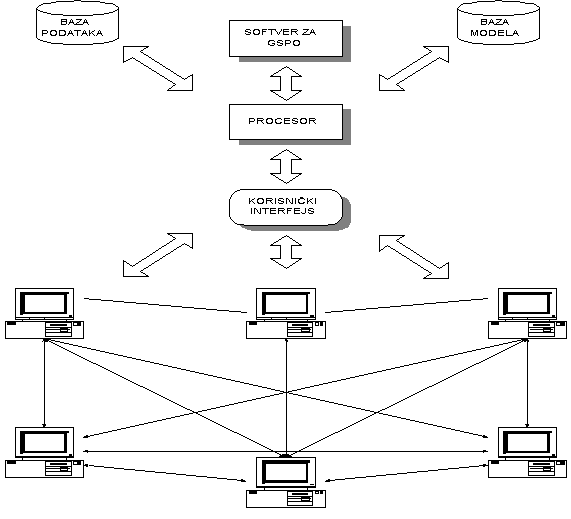
\includegraphics[width=0.85\linewidth]{slike/01/01-18.png}
    \caption{Основна технологија ГСПО}
    \label{fig:01-14}
\end{figure}

Према (Сукновић, 2001) технологија ГСПО подељена је у три нивоа:

\begin{itemize}
  \item 1. ниво - подршка процесу,
  \item 2. ниво - подршка одлучивању,
  \item 3. ниво - правило „реда“, односи се на контролу времена, садржаја дискусије, правила гласања, итд.
\end{itemize}
ГСПО првог нивоа обезбеђују техничке карактеристике за уклањање уобичајених комуникационих баријера, као што су велики екрани за тренутно приказивање идеја, сумирање гласова, анонимно уношење идеја и преференци, размена електронских порука између чланова групе, итд.

ГСПО другог нивоа обезбеђује моделирање одлука и техника групног одлучивања у циљу смањивања несигурности. За разлику од ГСПО првог нивоа који је само комуникациони медиј, ГСПО другог нивоа представља његово знатно проширење.

ГСПО трећег нивоа карактеришу стандардни обрасци за комуникацију у групи. Ови системи укључују и савете експерата у вези са избором и креирањем правила која ће се користити током састанка.

Што је већи ниво ГСПО, технологија мора бити савременија, али је и утицај на природан процес доношења одлука у групи све већи.

\subsection{Структура групних система за подршку одлучивању}
Сложеност процеса групног одлучивања умногоме модификује стандардну процедуру употребе индивидуалних система за подршку одлучивању. Према (Bui, 1987), та модификација варира у шест типова комуникације корисника и СПО.

\begin{figure}[h]
    \centering
    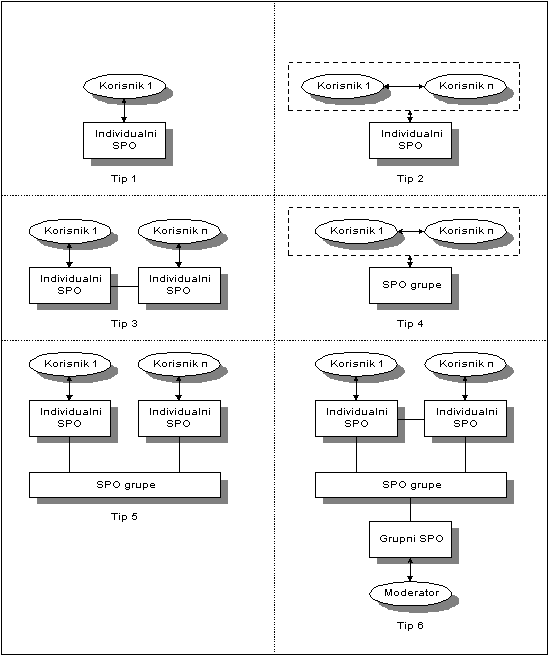
\includegraphics[width=0.85\linewidth]{slike/01/01-19.png}
    \caption{Типови комуникације корисник-СПО}
    \label{fig:01-15}
\end{figure}

Основни елементи који прате сваку развијену апликацију ГСПО су брзина реализације процеса групног одлучивања и тачност добијеног решења. Према (Сукновић, 2001), постоји пет варијанти структура одлучивања. Показало се да је структура звезда најефективнија код решавања структурираних и полуструктурираних проблема. Док структура точак највише одговара за неструктуриране и креативне ситуације одлучивања.

\begin{figure}[h]
    \centering
    
\includegraphics[width=0.85\linewidth]{slike/01/01-32.png}
    \caption{Могуће структуре одлучивања употребом ГСПО}
    \label{fig:01-16}
\end{figure}

\subsection{Пример архитектуре ГСПО и процеса одлучивања уз помоћ ГСПО}
Према (Bui, 1987), имплементација ГСПО може се базирати на моделима вишекритеријумског одлучивања. Тако ГСПО представља мрежу процесно оријентисаних индивидуалних СПО. Сваки учесник групног процеса одлучивања има сопствени СПО чија се база модела заснива методама и моделима вишекритеријумског одлучивања.

\begin{figure}[h]
    \centering
    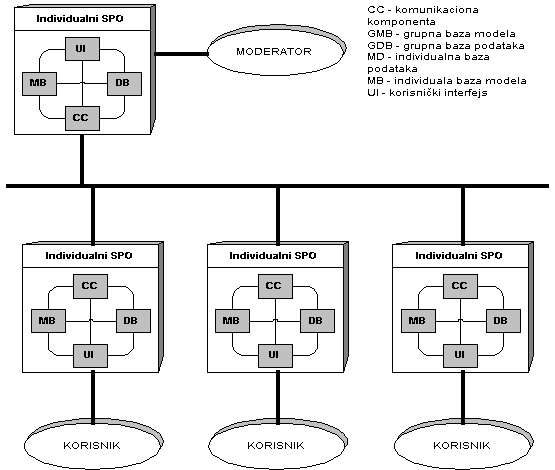
\includegraphics[width=0.85\linewidth]{slike/01/01-03.png}
    \caption{Могућа архитектура ГСПО - Тип 6 (Bui, 1987)}
    \label{fig:01-17}
\end{figure}

\begin{figure}[h]
    \centering
    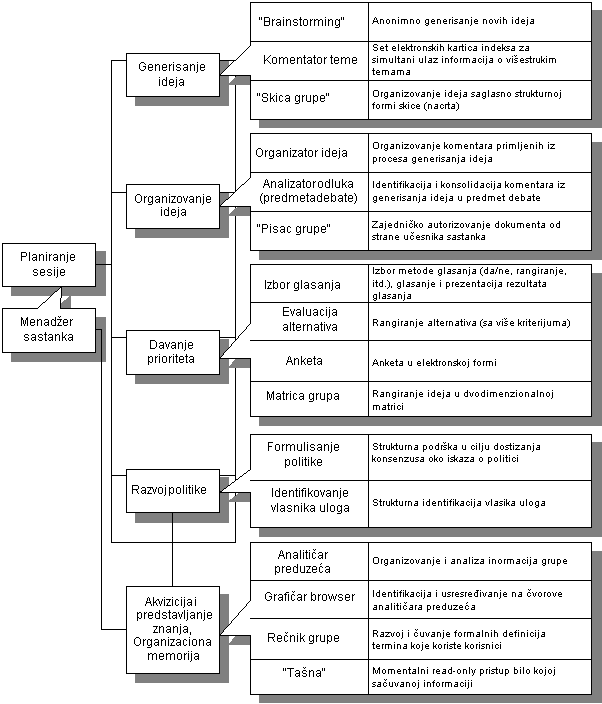
\includegraphics[width=0.85\linewidth]{slike/01/01-11.png}
    \caption{Неопходни модули рада развијене ГСПО апликације}
    \label{fig:01-18}
\end{figure}

\begin{figure}[h]
    \centering
    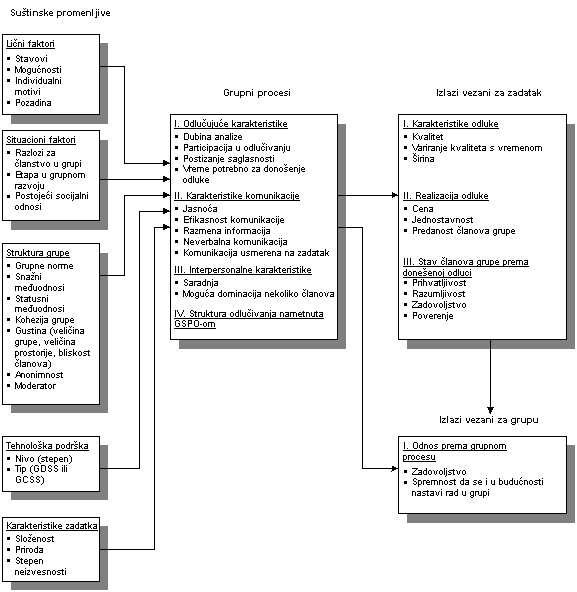
\includegraphics[width=0.85\linewidth]{slike/01/01-15.png}
    \caption{Улазне, процесне и излазне променљиве ГСПО}
    \label{fig:01-19}
\end{figure}

\subsection{Улога и задатак групе у формирању ГСПО}
Задатак са којим се сусреће група мора да буде покретачка снага за дизајнирање ГСПО. Карактеристике задатка одређују потребу за информацијама и начин комуникације у групи која доноси одлуке.

Главни циљеви групе према (Сукновић, 2001) су:

\begin{itemize}
  \item генерисање идеја и алтернатива (креативни задаци захтевају генерисање нових идеја, док плански задаци захтевају генерисање планова оријентисаних на алтернативе);
  \item избор алтернатива (решавање и примена решења подразумева избор најприхватљивије алтернативе);
  \item преговарање о алтернативама (сазнајно-конфликтни задаци подразумевају приближавање супротстављених гледишта).
\end{itemize}
Предности примене ГСПО према (Сукновић, 2001) су:

\begin{itemize}
  \item олакшавају и поједностављују унос и приказ идеја свих чланова групе,
  \item повећавају брзину процене идеја,
  \item обезбеђују техничку подршку за активности креативног мишљења,
  \item поседују могућност избора исправног решења,
  \item повећавају ефективност решења у задацима преговарања.
\end{itemize}
Са растом притиска да се одлуке доносе у групама, јавља се потреба за развојем и изучавањем система за групно доношење одлука, ослоњених на јаку подршку савремених информационо-комуникационих технологија.

У претходним потпоглављима приказани су системи који подржавају индивидуално и групно доношење одлука – СПО, ЕС и ГСПО. Сви ови системи имају заједнички циљ: да доносиоцу одлуке омогуће приступ потребном знању за доношење исправне управљачке пословне одлуке. На самом почетку овог поглавља дефинисана је пословна интелигенција као скуп технологија, организационих правила и знања удружен у генерисању знања за доношење одлуке. Такође, у потпоглављу о експертним системима, детаљно је описано како се знање чува и користи у базама знања. Међутим, до сада није прецизно дефинисано шта је заправо знање у контексту пословне интелигенције, који облици знања постоје и како се знање открива и систематизује. Управо та питања су тема наредних потпоглавља, у којима се формализује појам знања, уводе узори као носиоци знања и представља целокупан модел пословне интелигенције.

\section{Знање у пословној интелигенцији}
Често се корисницима система пословне интелигенције обећава да ће им системи пословне интелигенције (ПИ) пронаћи знање, које ће омогућити корисницима да боље доносе одлуке. Корисници, са друге стране, често нису ни свесни шта је знање, а ни аналитичари који помажу у откривању знања често не знају шта заправо траже.

У наставку се покушава да се донекле боље објасни шта је знање у пословној интелигенцији, како га препознати и презентовати да би било употребљиво и да би било коришћено у пословном процесу. Сврха система ПИ је пословно обавештавање (кроз управљачке извештаје, откривене законитости, управљачке моделе итд.) са циљем пружања ДО знања које могу довести до одлуке за решавање одређеног пословног проблема.

\section{Врсте знања}
Основа за доношење пословних одлука јесте знање. Циљ подршке одлучивању је предлагање акције (одлуке) коју ДО треба да спроведе када се јави проблем у одређеном контексту.

Око дефиниције знања не постоји општа сагласност. Дефиниција коју ћемо користити за објашњавање знања у пословној интелигенцији је по (Tiwana, 2000):

\textbf{Информација са акцијом расположива у правом формату, у право време и на правом месту за одлучивање.}

Знање је увек везано за контекст, а то значи да знање које важи у одређеном контексту, не мора да важи у другом контексту. Знање представља тројку проблема, контекста и решења. Решење представља предлог акције, који се предлаже ДО.

За знање важи да:

1. Поседовање знања је предуслов доношења исправних управљачких пословних одлука;

2. Знање у себи садржи компоненту акције (решења);

3. Знање је везано за контекст;

4. Знање може да се представи тројком: проблем, контекст и решење;

5. Знање представља прихватљиво решење одређеног проблема, које најчешће није оптимално, и

6. Свако знање тражи одређену емпиријску потврду.

У Табели~\ref{tab:01-3} приказане су неке дефиниције знања на које често може да се наиђе у литератури.

\begin{table}[h]
\centering
\begin{adjustbox}{max width=\textwidth}
\begin{tabular}{|l|l|}
\hline
\textbf{Дефиниција} & \textbf{Аутор} \\
\hline
Способност претварања информација и података у ефективну акцију & (Applehans et al., 1999) \\
\hline
Значајне везе које људи праве у својим умовима између информација и њихове примене у акцију у специфичном контексту & (Dixon, 2000) \\
\hline
Флуидни микс уоквиреног искуства, вредности, контекстуалних информација и експертског увида & (Firestone, 2003) \\
\hline
Знање је информација која је прошла процес валидације & (Firestone, 2003) \\
\hline
Идејна конструкција генерисана преко људског ума & (Housel \& Bell, 2001) \\
\hline
Организациони ресурс састављен од суме онога што се зна & (Holsapple et al., 1996) \\
\hline
Систематизоване и структуриране информације специфичне намене & (Johanessen et al., 2001) \\
\hline
Информација чија је валидност успостављена кроз тестове и доказе & (Liebeskind, 1996) \\
\hline
\end{tabular}
\end{adjustbox}
    \caption{Разне дефиниције знања}
    \label{tab:01-3}
\end{table}

Знање може да се подели на процедурално, дескриптивно, семантичко и епизодно према (Awad \& Ghaziri, 2004).

\textbf{Процедурално знање}

Објашњава процедуру решавања одређеног проблема. Карактеристика овог знања је да оно објашњава како се решава одређени проблем. Ово знање одговара на питање „Како?“, али не и на питање „Зашто?“.

\textbf{Дескриптивно знање}

Описује са више детаља одређени проблем са циљем да се боље објасне појмови везани за конкретну проблематику. Овом знању недостаје организација знања у облику проблем, контекст, решење.

\textbf{Семантичко знање}

Знање код кога су уочене везе и зависности које владају између делова проблема, контекста и решења. Представља надоградњу дескриптивног знања.

\textbf{Епизодно знање}

Састављено из низа повезаних искуствених записа, тј. случајева. Епизоде су одређена искуствена знања. Епизодно знање садржи компоненту акције и представља заправо низ епизода између којих постоји одређени редослед. Епизодно знање је најупотребљивије за доношење пословних одлука.

Циљ је да свако знање пређе пут од процедуралног и дескриптивног до епизодног, да би се на крају проблем који захтева епизодно знање, могао решавати на процедуралан начин.

Претходно описана подела знања може да се објасни на примеру рецепта за пудинг.

\textbf{Процедурално знање (рецепт за пудинг):}

Припремите 0,5 л млека. Одмерите 1 дл хладног млека, додајте садржај кесице и мешајте док маса не постане глатка. Преосталу количину млека засладите са три кашике шећера и загрејте до кључања. Склоните са ватре, умешајте припремљену масу и кувајте два минута уз непрестано мешање. Врелу масу сипајте у влажне посуде и оставите да се пудинг стегне и охлади.

\textbf{Дескриптивно знање:}

Маса је глатка када је смеса за пудинг разложена у маси млека, тј. када је растопљена и не постоје грануле. Врела маса се сипа у влажне посуде да се пудинг не би залепио за ивице посуде.

\textbf{Семантичко знање:}

Постоји веза између ефективности мешања смесе са температуром млека. Маса за пудинг се боље размућује у хладном млеку. Постоји веза између лепљења смесе пудинга за зид посуде и влажности посуде.

\textbf{Епизодно знање (четири епизоде):}

1. Раздвој у делове -> 2. Корак по корак -> 3. Направити прелаз -> 4. Расподелити равномерно

\begin{figure}[h]
    \centering
    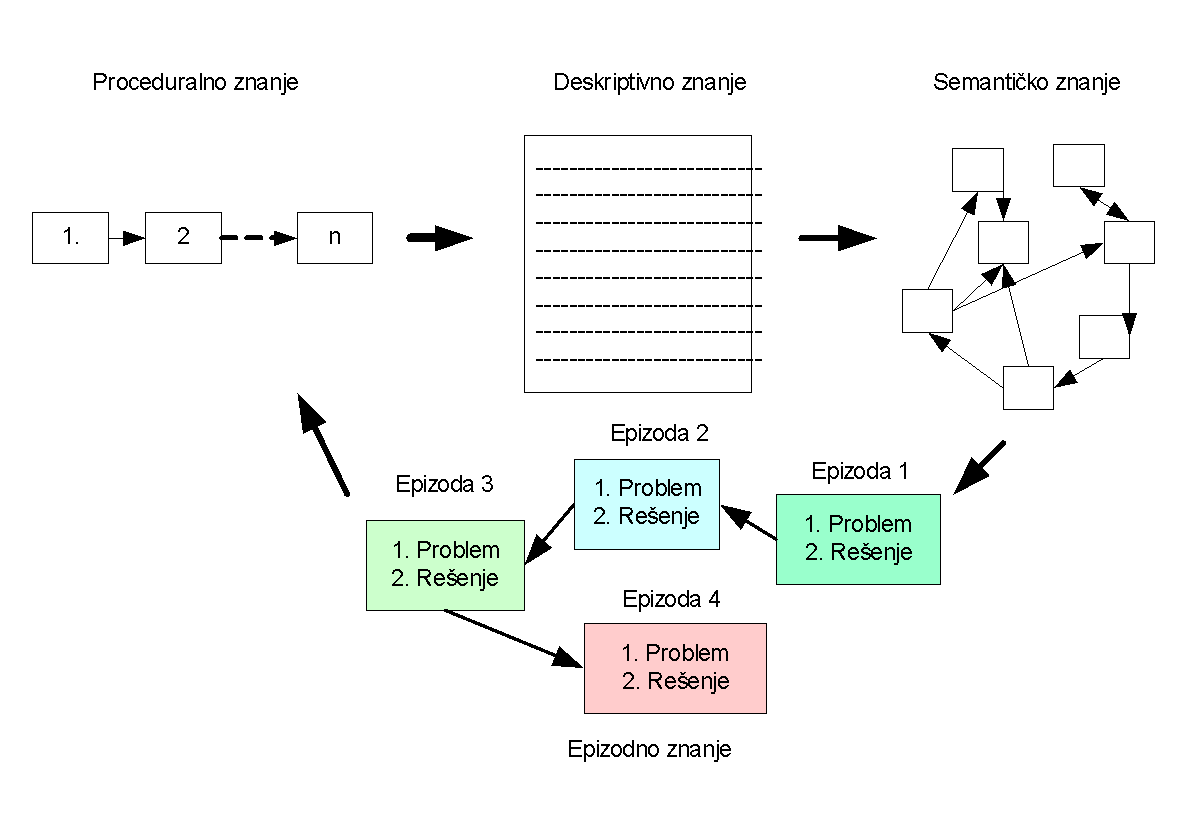
\includegraphics[width=0.85\linewidth]{slike/01/01-04.png}
    \caption{Од процедуралног до епизодног знања и назад}
    \label{fig:01-20}
\end{figure}

Једна од најпознатијих подела знања у свету менаџмента знања је подела на експлицитно и прећутно (подразумевано) знање.

\textbf{Експлицитно знање}

Знање садржано у књигама, документима, извештајима, табелама и сл. Може једноставно да се формализује, представи и сачува у електронској форми.

\textbf{Прећутно знање}

Онај део знања појединаца који се теже формализује. То је знање које је прошло искуствену проверу. Најзанимљивији део прећутног знања је експертско знање које има велику вредност.

Савремени развој вештачке интелигенције, посебно великих језичких модела, отвара нове могућности за формализацију и коришћење прећутног знања. Ови модели су обучени на огромним количинама текста и могу да асистирају у процесу екстернализације знања, генерисању извештаја и подршци одлучивању на начине који раније нису били могући.

\begin{figure}[h]
    \centering
    
\includegraphics[width=0.85\linewidth]{slike/01/01-24.png}
    \caption{Веза између контекста и разумевања}
    \label{fig:01-21}
\end{figure}

Податак је основни градивни елемент информације и знања. Информација је структура (организован податак). Знање има сложенију структуру од информације, јер садржи и компоненту решења одређеног проблема.

\textbf{Знање садржи компоненту акције. То омогућава подршку одлучивању. Знање је, због тога, основа подршке пословном одлучивању.}

Један облик представљања знања јесте узор. Узор је носилац знања, али је и градивни елемент знања.

\begin{figure}[h]
    \centering
    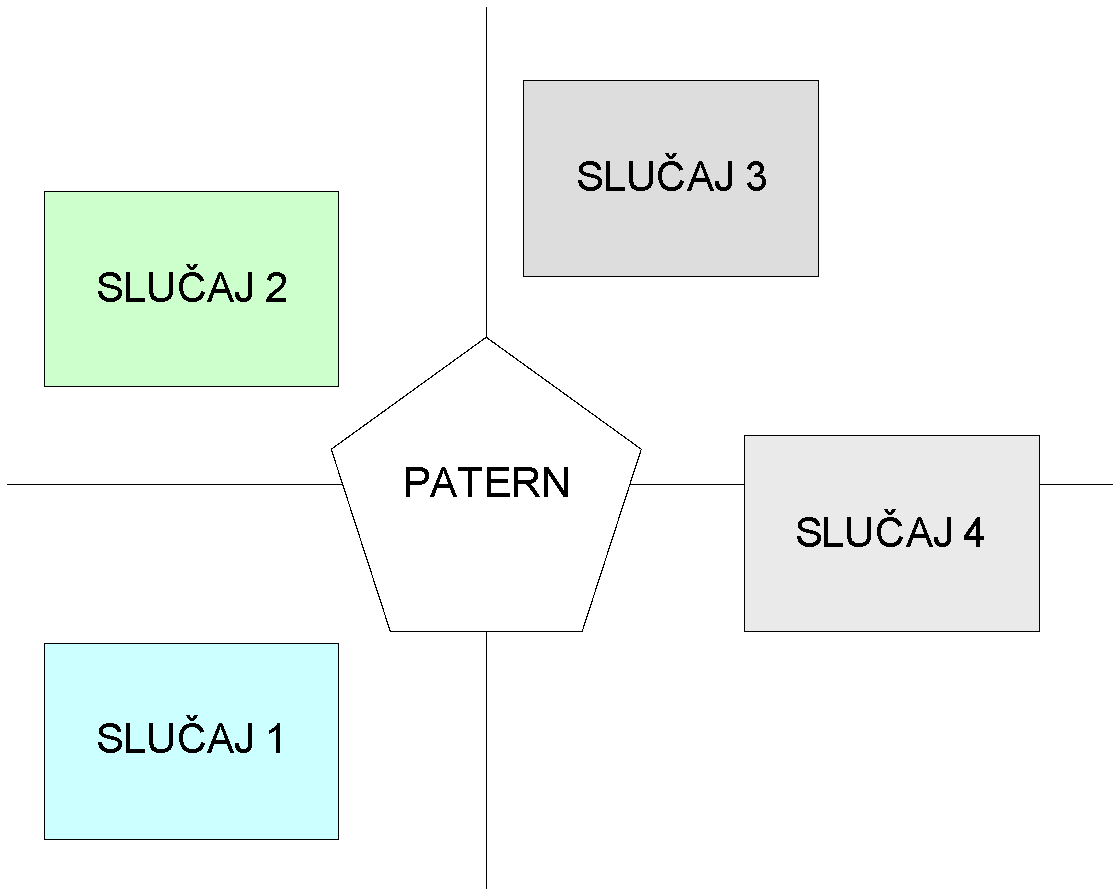
\includegraphics[width=0.85\linewidth]{slike/01/01-21.png}
    \caption{Случајеви теже узорима}
    \label{fig:01-22}
\end{figure}

\section{Узори}
По (Делибашић, 2007), узори представљају искуствено доказана решења за проблеме у одређеном контексту. Могу да се представе тројком \{проблем, контекст, решење\}. За разлику од случајева и других облика знања који имају сличну форму, узори су прошли искуствену валидацију.

Знање експерта може да се моделира преко узора. Сваки експерт је током свог процеса учења савладао одређени број узора који га чине експертом у тој области.

Данас се узори проучавају највише у софтверском инжењерству. Примећено је да се одређена искуствена проверена решења понављају у различитим софтверима, те да их је могуће уочити и делити са осталим софтверским инжењерима.

Идеја творца узор покрета Кристофера Александера (Alexander, 1964, 2002) је да нађе фундаменталне законитости по којима природа и људи стварају.

\begin{figure}[h]
    \centering
    
\includegraphics[width=0.85\linewidth]{slike/01/01-05.png}
    \caption{Мост храма Исе Јингу у Јапану}
    \label{fig:01-23}
\end{figure}

\begin{figure}[h]
    \centering
    
\includegraphics[width=0.85\linewidth]{slike/01/01-07.png}
    \caption{Џамија Масјид-и-Схах у Ирану}
    \label{fig:01-24}
\end{figure}

Ако се у области као што је архитектура могу утврдити законитости по којима треба градити и решавати проблеме, тада се и у свим осталим областима може урадити исто.

Два су појма кључна за схватање Александерове теорије. То су целина и узор. Александер изводи следеће закључке:

1. Узори су искуствена решења.

2. Узори се надопуњују: постојање и функционисање једног узора утиче на други узор.

3. Узори су састављени од узора и

4. Целина добија своју животност с обзиром на густину и интензитет узора који постоје унутар ње.

Скуп узора који чине једно решење једног проблема назива се узор језик. У (Winn \& Calder, 2002) су предложене неке особине које треба да има узор:

1. Треба да буде алат направљен за решавање одређеног проблема.

2. Треба да повезује различите нивое апстракције решења.

3. Садржи и функционалне и нефункционалне особине.

4. Препознатљивост у решењу.

5. Решава битне одлуке код пројектовања решења.

6. Представља део узор језика.

7. Искуствено је проверен.

8. Везан је за одређени домен.

9. Представља значајну идеју.

\section{Узори одлучивања}
Код пројектовања универзитетског насеља Ејшин код Токија пројектанти су пошли од својих корисника и анализирајући навике и потребе корисника, архитекте су смислиле начин како да изграде насеље које у саме грађевине уноси функционалности које подржавају живот класичног јапанског студента.

\begin{figure}[h]
    \centering
    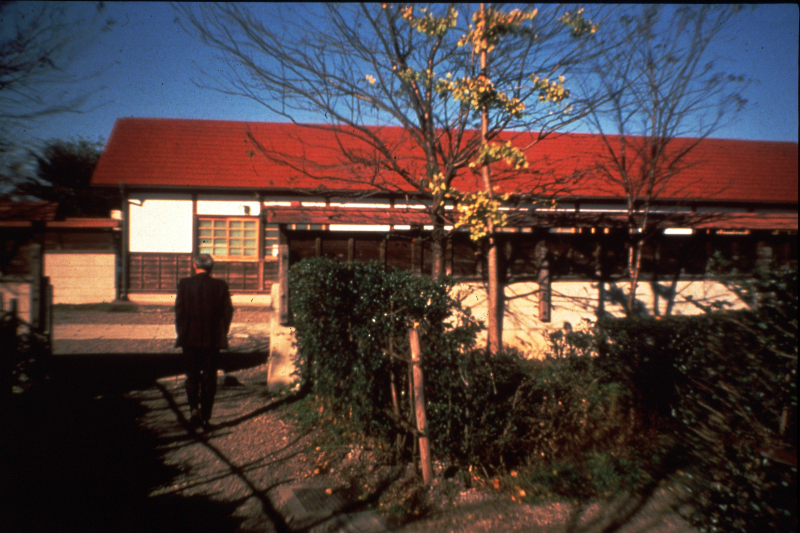
\includegraphics[width=0.85\linewidth]{slike/01/01-17.png}
    \caption{Слике универзитетског насеља (Ејшин кампус)}
    \label{fig:01-25}
\end{figure}

Ако се направи аналогија са одлучивањем, може да се каже да је већина алгоритама за подршку одлучивању направљена од стране научника који не познају већину захтева корисника.

Пример једног узора у Коплиеновој форми:

\textbf{Ко испадне из строја, остаје ван строја.}

1. Контекст: Узор се користи у редно везаним системима.

2. Проблем: Како да систем остане ефикасан када један члан кочи цео систем?

3. Силе: Снага редно везаног система је једнака снази најслабијег објекта.

4. Решење: Избацити објекат из система, вратити га на крај реда.

5. Резултујући контекст: Избацивањем објекта који успорава систем, систем функционише ефикасније.

\subsection{Четири узора одлучивања и процес откривања знања}
Четири узора која се јављају у процесу одлучивања су:

1. Divide et Impera (Подели и владај), Анализа,

2. Додели заједничку вредност,

3. Сви као један (Агрегација) и

4. Анализа.

\textbf{Divide et Impera (подели и владај) - Анализа}

Један од најраспрострањенијих узора у природи. Сваки проблем који се јавља у животу, обично је такав да треба да се растави на мање делове да би био савладив. Код подршке одлучивања и пословне интелигенције, овај узор има велику улогу у дефинисању структуре проблема која је управљива.

\begin{figure}[h]
    \centering
    
\includegraphics[width=0.85\linewidth]{slike/01/01-06.jpg}
    \caption{Зид који треба савладати}
    \label{fig:01-26}
\end{figure}

\textbf{Додели заједничку вредност - Нормализација}

Овим узором, који се често зове и нормализација, свим подацима се додељују заједничка обележја. Сви подаци који чине базу података за одлучивање добијају заједничку меру преко којих сви подаци могу да се изразе. Ово је потребно ради остваривања могућности да се упоређују подаци.

\begin{figure}[h]
    \centering
    
\includegraphics[width=0.85\linewidth]{slike/01/01-10.jpg}
    \caption{Униформисани војници}
    \label{fig:01-27}
\end{figure}

\textbf{Сви као један (Агрегација) - Синтеза}

Узор који представља функцију која из података извлачи агрегације, тј. решење на основу којих може да се доноси одлука. Ово је синтетичка фаза добијања знања, док је „Дивиде ет импера“ аналитичка фаза, а „Додели заједничку вредност“ повезује аналитичку и синтетичку фазу процеса откривања знања.

\begin{figure}[h]
    \centering
    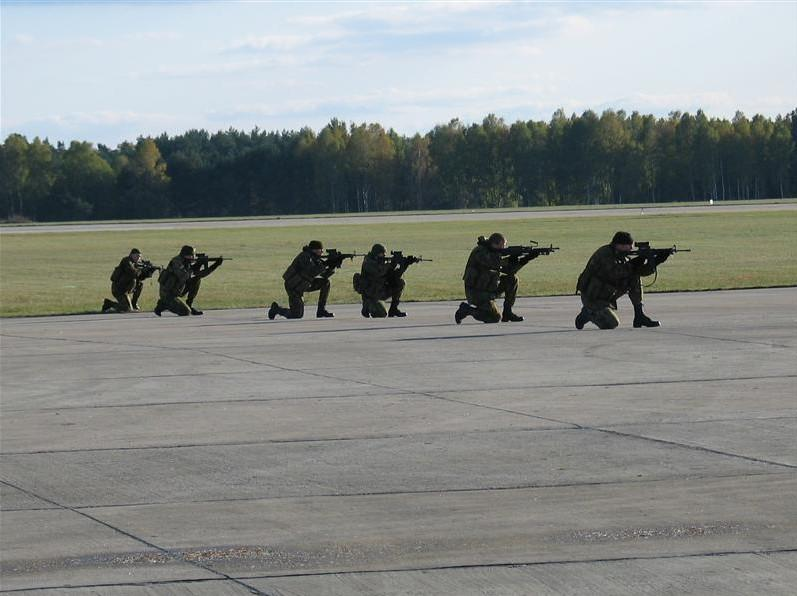
\includegraphics[width=0.85\linewidth]{slike/01/01-08.jpg}
    \caption{Војници у положају за гађање}
    \label{fig:01-28}
\end{figure}

\textbf{Евалуација}

Последњи, али можда и најважнији узор одлучивања. Представља узор који унапређује систем одлучивања. Један је од кључних узора у одлучивању јер показује колико је откривено решење добро или не.

\begin{figure}[h]
    \centering
    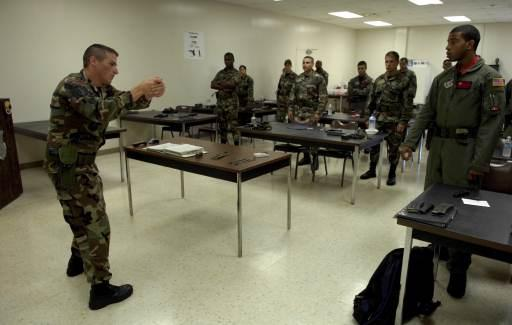
\includegraphics[width=0.85\linewidth]{slike/01/01-14.jpg}
    \caption{Евалуација и припрема за нове задатке}
    \label{fig:01-29}
\end{figure}

\begin{figure}[h]
    \centering
    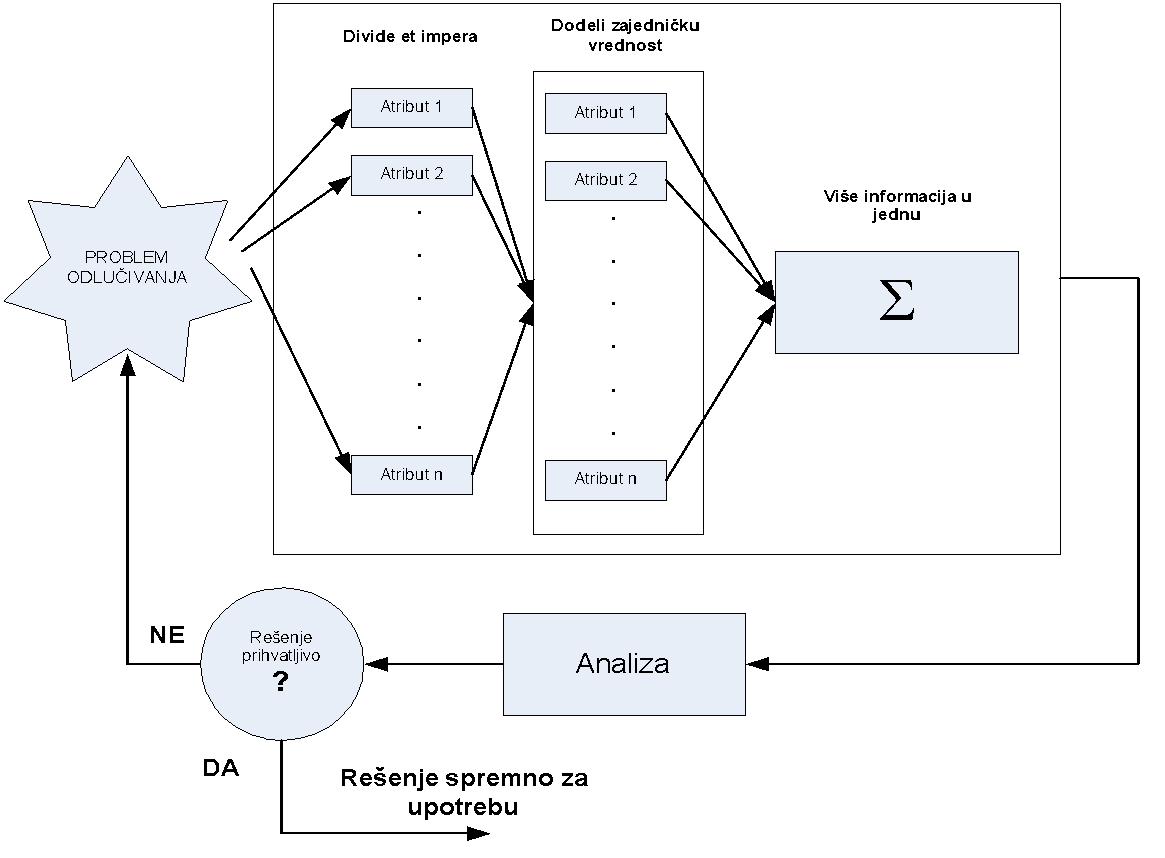
\includegraphics[width=0.85\linewidth]{slike/01/01-01.png}
    \caption{Процес одлучивања преко узора}
    \label{fig:01-30}
\end{figure}

Када постоји проблем, прво се покреће узор „Divide et Impera“. Потом се ради „Додели заједничку вредност“ и „Сви као један“. На крају се узором „Евалуација“ проверава колико је добијено решење добро. Уколико је решење (откривено знање) прихватљиво, процес се зауставља, а уколико не улази се у нову итерацију.

\section{Закључак: Модел пословне интелигенције}
У овом поглављу су представљени системи за подршку одлучивању (СПО и ЕС), системи за подршку групном одлучивању (ГСПО), као и појам знања у пословној интелигенцији. Сви ови концепти конвергирају у моделу пословне интелигенције који следи.

Са циљем да се ДО омогући да доноси исправне управљачке пословне одлуке, могу да се искористе све дисциплине описане у овој књизи.

\begin{figure}[h]
    \centering
    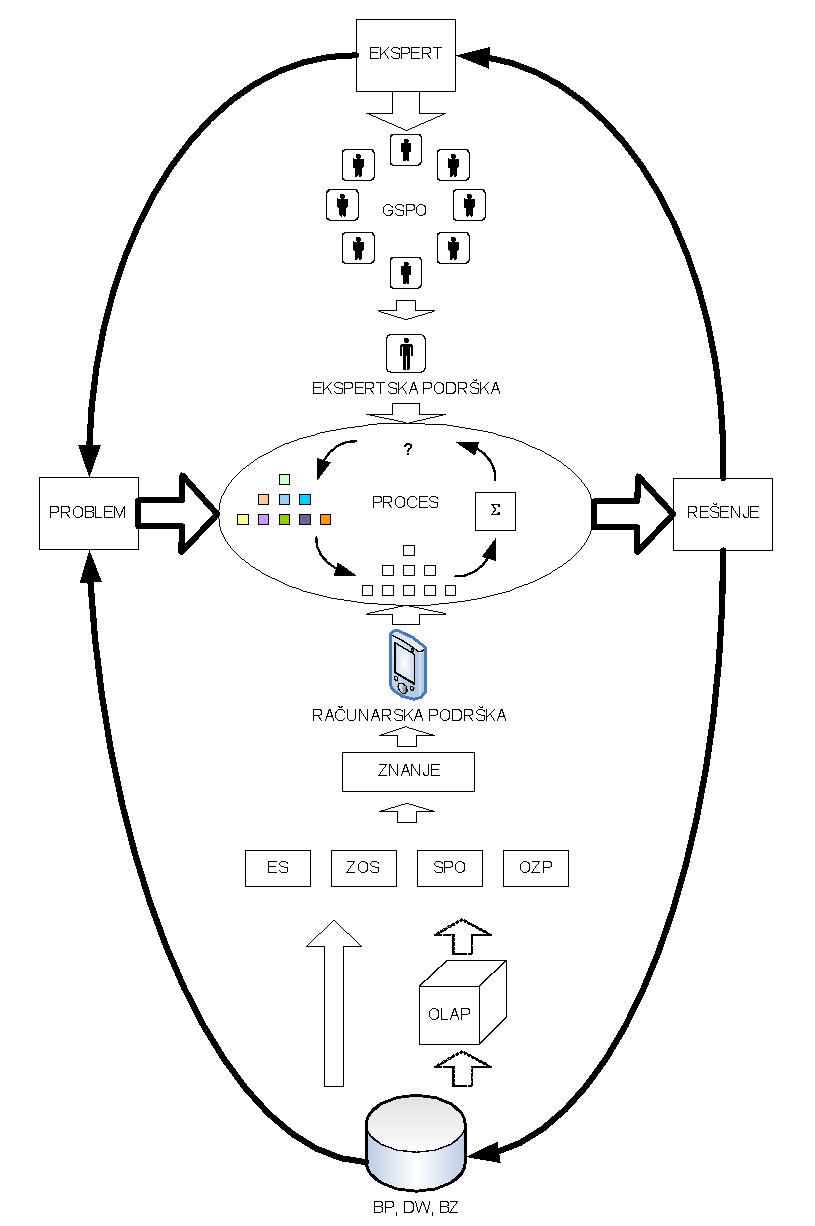
\includegraphics[width=0.85\linewidth]{slike/01/01-02.png}
    \caption{Модел пословне интелигенције}
    \label{fig:01-31}
\end{figure}

Основни циљ ДО је да одређени проблем који се јавља у пословном процесу организације реши у што краћем времену на што бољи начин. То може да уради уколико поседује знање за доношење одлуке.

Централни део слике представља процес откривања знања који је описан преко четири фундаментална узора одлучивања и то „Divide et Impera“, „Додели заједничку вредност“, „Сви као један“ и „Евалуација“.

Модел ПИ пружа ДО подршку у процесу доласка до знања користећи експертску и рачунарску помоћ. Са експертске стране, ДО стоји на располагању или подршка групе или експертска подршка. Сваки пут када група или експерт реше одређени проблем они тиме знање које поседују унапређују.

Са друге стране, рачунарска подршка се заснива на подацима који се прикупљају у базама и складиштима која садрже најзанимљивије податке за анализу и базама знања (БЗ) које чувају ускладиштено знање експерата у одређеној области.

Над складиштем података је могуће изградити ОЛАП коцку. Над ОЛАП коцком је могуће спроводити ОЗП, изградити систем ЗОС. Над базом података и складиштем података је могуће развити систем ЗОС или спроводити ОЗП. Над базом знања је могуће развити експертни систем. СПО је могуће развити над неким моделима које је открио ЗОС или неким другим искуствено провереним моделима које је могуће користити у организацији.

Пословна интелигенција би требало да буде интегрални део сваког информационог система организације. Из тог разлога би све одлуке које се спроводе требало чувати у одговарајућим базама. Ово би омогућило да се знање ефикасно користи и да организација користи пун потенцијал својих кадрова и својих података.

У данашње време, овај модел се проширује новим компонентама. Поред класичних база података и складишта података, организације користе и језера података (Data Lake) за чување неструктурираних података. Алгоритми машинског учења и дубоко учење (Deep Learning) допуњују или замењују класичне ОЗП алгоритме. Системи вештачке интелигенције, укључујући велике језичке моделе, омогућавају конверзацијски приступ подацима где корисник може постављати питања на природном језику и добијати одговоре засноване на анализи података организације. Самоуслужни БИ алати демократизују приступ аналитици, чинећи је доступном ширем кругу запослених у организацији.

Пословна интелигенција је област која се константно развија. Кључни савремени трендови у ПИ укључују:

1. Самоуслужна пословна интелигенција (Self-Service BI): Алати попут Power BI, Tableau и Looker омогућавају крајњим корисницима да сами креирају извештаје и визуализације без помоћи ИТ одељења.

2. Аналитика у облаку (Cloud Analytics): Све више организација мигрира своје БИ системе у облак (AWS, Azure, Google Cloud), чиме се смањују трошкови инфраструктуре и повећава скалабилност.

3. Вештачка интелигенција и машинско учење: Алгоритми машинског учења, укључујући дубоко учење (Deep Learning) и велике језичке моделе (Large Language Models - LLM), аутоматизују откривање законитости у подацима и пружају предиктивну аналитику.

4. Аналитика у реалном времену: Системи за обраду токова података (енг. Stream Processing) омогућавају доношење одлука на основу података који пристижу у реалном времену.

5. Демократизација података: Тренд да сви запослени у организацији имају приступ релевантним подацима и алатима за њихову анализу, а не само специјализовани аналитичари.

\section{Литература}
[1] Делибашић Б (2007) Формализација процеса пословног одлучивања преко патерна, докторска дисертација, ФОН, Београд.

[2] Делибашић Б, Сукновић М, Јовановић М (2009) Алгоритми машинског учења за откривање законитости у подацима, ФОН, Београд.

[3] Сукновић М, Делибашић Б (2010) Пословна интелигенција и системи за подршку одлучивању, Факултет организационих наука, ISBN 978-86-7680-206-7.

[4] Сукновић М, Делибашић Б, Јовановић М, Вукићевић М, Радовановић С (2021) Одлучивање, ФОН, ISBN 978-86-7680-370-5.

[5] Сукновић М (2001) Развој методологије подршке групном одлучивању, докторска дисертација, ФОН, Београд.

[6] Alexander C (1964) Notes on the Synthesis of Form, Harvard University Press.

[7] Alexander C (2002) The Nature of Order Book 1: The Phenomenon of Life, The Center for Environmental Structure, Berkeley California.

[8] Awad E, Ghaziri H (2004) Knowledge Management, Prentice Hall.

[9] Azvine B, Cui Z, Nauck DD, Majeed B (2006) Real time business intelligence for the adaptive enterprise, International Conference on Enterprise Computing.

[10] Bennett J (1983) Building decision support systems, Addison-Wesley, Massachusetts.

[11] Bui TX (1987) Cooperative Co-oP group decision support systems for multiple criteria group decision making, Springer-Verlag, Berlin Heidelberg.

[12] DeSanctis G, Gallupe B (1987) A Foundation For The Study of Group Decision Support Systems, Management Science Vol. 33 No. 5.

[13] Dixon N (2000) Common Knowledge, Harvard Business School Press.

[14] Firestone J (2003) Enterprise Information Portals and Knowledge Management, Butterworth-Heinemann.

[15] Holsapple C, Whinston W, Andrew B (1996) Decision Support Systems - A Knowledge-Based Approach, West Publishing Company.

[16] Housel T, Bell AA (2001) Measuring and Managing Knowledge, McGraw-Hill.

[17] Johannessen J, Olaisen J, Olsen B (2001) Mismanagement of Tacit Knowledge, International Journal of Information Management, Vol. 21, No. 1.

[18] Lawton G (2006) Making business intelligence more useful.

[19] Leigh WE, Doherty ME (1986) Decision Support and Expert Systems, South-Western Publishing Company, Cincinnati, Ohio.

[20] Liebeskind J (1996) Knowledge, Strategy and the Theory of the Firm, Strategic Management Journal.

[21] Meader CL, Guyote MJ, Keen PGW (1984) Setting Priorities for DSS Development, MIS Quarterly 8, str. 117-131.

[22] Simon HA (1945) Administrative Behavior, Free Press, New York.

[23] Sprague RH, Carlson ED (1982) Building Effective Decision Support Systems, Prentice Hall, Englewood Cliffs.

[24] Roland RJ (1982) A model of organizational variables for DSS, Data Base 12, str. 63-72.

[25] Theireuf RJ (1989) Group decision support systems for effective decision making, Quorum Book.

[26] Tiwana A (2000) The Knowledge Management Toolkit, Prentice Hall.

[27] Turban E, Carlson JG (1989) Interactive Visual Decision-Making, U knjizi: Decision Support Systems, Prentice Hall, New Jersey.

[28] Turban E, Aronson JE, Liang TP, Sharda R (2006) Decision Support and Business Intelligence Systems, Prentice Hall.

[29] Winn T, Calder P (2002) Is this a pattern?, IEEE Software.

[30] Zelenny M (1982) Multiple Criteria Decision Making, McGraw-Hill, New York.
